% Spacetime Engineering: master document.
% Build with `make` (latexmk, pdfLaTeX, biber). Figures are standalone files in
% figures/src, built by `make figures`. One chapter:
%   make chapter CH=chapters/ch02-spacetime-geometry

\documentclass[
  paper=letter,
  fontsize=10pt,
  twoside=true,
  twocolumn=true,
  open=right,
  chapterprefix=false,
  numbers=noenddot,
  bibliography=totoc,
  index=totoc,
]{scrbook}

% Packages. hyperref and cleveref come last.

\usepackage[
  letterpaper,
  inner=0.8in, outer=0.7in,
  top=0.9in, bottom=0.95in,
  columnsep=0.3in,
  headheight=14pt, headsep=18pt, footskip=30pt,
]{geometry}

\usepackage{mathtools}

\usepackage[T1]{fontenc}
\usepackage{newpxtext}
\usepackage[varbb]{newpxmath}
\usepackage[semibold,scale=0.95,lining]{sourcesanspro}
\usepackage[final]{microtype}
\linespread{1.04}

\usepackage{bm}
\usepackage[separate-uncertainty=true,per-mode=symbol]{siunitx}

\usepackage{etoolbox}
\usepackage{enumitem}
\usepackage{booktabs}
\usepackage{tabularx}
\usepackage{array}
\usepackage{multicol}
\usepackage{graphicx}
\graphicspath{{figures/}}
\usepackage{xcolor}
% Palette shared by the book and by the standalone figures in figures/src.
% One main hue (blue), one accent (orange), and a few roles used sparingly.

\definecolor{seblue}{HTML}{1D5B8F}    % headings, worked examples, main curves
\definecolor{seblueDark}{HTML}{123E63}
\definecolor{seorange}{HTML}{DC7A26}  % thought experiments, light and light cones
\definecolor{seteal}{HTML}{1F8577}    % checks, travellers and ships
\definecolor{sered}{HTML}{C0392B}     % negative energy, tension, violations
\definecolor{seviolet}{HTML}{5E548E}  % going deeper
\definecolor{sesand}{HTML}{8C6A3F}    % history
\definecolor{segray}{HTML}{6B7480}    % axes, guides, secondary labels
\definecolor{selight}{HTML}{D5DAE1}   % grids and faint rules

\usepackage{tikz}
\usetikzlibrary{arrows.meta,positioning,calc}
\usepackage[most]{tcolorbox}
\usepackage{fontawesome5}
\usepackage{csquotes}
\usepackage{scrlayer-scrpage}
\usepackage{scrhack}

\usepackage[
  backend=biber,
  style=authoryear-comp,
  maxcitenames=2,
  maxbibnames=10,
  minbibnames=3,
  giveninits=true,
  uniquename=init,
  uniquelist=false,
  dashed=false,
  sortcites=true,
  date=year,
  doi=true,
  eprint=true,
  url=false,
  isbn=false,
]{biblatex}

% The shared bibliography carries provenance notes for the repository's
% evidence review; the book's reference list leaves them out.
\DeclareSourcemap{
  \maps[datatype=bibtex]{
    \map{\step[fieldset=note, null]\step[fieldset=addendum, null]}
  }
}

\usepackage{imakeidx}
\makeindex[intoc]

\usepackage[hidelinks,bookmarksnumbered,pdfusetitle]{hyperref}
\usepackage[nameinlink,capitalise,noabbrev]{cleveref}

% Page layout, headings and running heads.
%
% Chapters are numbered. Topics inside a chapter carry descriptive, unnumbered
% headings; equations, figures, examples and problems are numbered by chapter.

\setcounter{secnumdepth}{\chapternumdepth}
\setcounter{tocdepth}{\sectiontocdepth}

\counterwithin{equation}{chapter}
\counterwithin{figure}{chapter}
\counterwithin{table}{chapter}

% ---------------------------------------------------------------------------
% Headings
\setkomafont{disposition}{\sffamily\bfseries}
\setkomafont{part}{\sffamily\bfseries\fontsize{30}{36}\selectfont}
\setkomafont{partnumber}{\sffamily\mdseries\fontsize{18}{22}\selectfont\color{seblue}}
\setkomafont{chapter}{\sffamily\bfseries\fontsize{25}{30}\selectfont}
\setkomafont{section}{\sffamily\bfseries\fontsize{13}{16}\selectfont\color{seblue}}
\setkomafont{subsection}{\sffamily\bfseries\normalsize\color{black!82}}
\setkomafont{paragraph}{\sffamily\bfseries\small\color{black!82}}

\RedeclareSectionCommand[
  beforeskip=0pt, afterskip=1.4\baselineskip,
]{chapter}
\RedeclareSectionCommand[
  beforeskip=1.5\baselineskip plus 0.5\baselineskip minus 0.2\baselineskip,
  afterskip=0.55\baselineskip plus 0.1\baselineskip,
]{section}
\RedeclareSectionCommand[
  beforeskip=1.0\baselineskip plus 0.3\baselineskip minus 0.1\baselineskip,
  afterskip=0.35\baselineskip,
]{subsection}
\RedeclareSectionCommand[
  beforeskip=0.6\baselineskip plus 0.2\baselineskip, afterskip=-0.6em,
]{paragraph}

% Chapter heads: a small label, a large number, the title and a rule. The
% chapter preamble (lead paragraph and goals) follows across both columns.
\makeatletter
\renewcommand*{\chapterformat}{\thechapter}
\renewcommand*{\chapterlinesformat}[3]{%
  \Ifstr{#1}{chapter}{%
    \IfArgIsEmpty{#2}{}{%
      {\normalfont\sffamily\small\color{segray}\textls[150]{\MakeUppercase{\chapapp}}\par}%
      {\normalfont\sffamily\fontsize{54}{50}\selectfont\color{seblue}#2\par}%
      \vspace{0.25\baselineskip}}%
    #3\par
    \vspace{0.3\baselineskip}%
    {\color{seblue}\rule{\linewidth}{0.9pt}}\par
  }{\@hangfrom{#2}{#3}}%
}
\makeatother

% ---------------------------------------------------------------------------
% Running heads: chapter on the left page, topic on the right.
\pagestyle{scrheadings}
\clearpairofpagestyles
\automark[section]{chapter}
\renewcommand*{\chaptermarkformat}{\thechapter\enskip}
\ohead{\headmark}
\ofoot*{\pagemark}
\ifoot*{\textcolor{segray}{Draft\enspace\today}}
\setkomafont{pageheadfoot}{\normalfont\sffamily\footnotesize\color{black!70}}
\setkomafont{pagenumber}{\normalfont\sffamily\bfseries\footnotesize\color{seblue}}
\renewcommand*{\chapterpagestyle}{plain.scrheadings}

% ---------------------------------------------------------------------------
% Captions
\setkomafont{captionlabel}{\sffamily\bfseries\color{seblue}}
\setkomafont{caption}{\small}
\setcapindent{0pt}
\renewcommand*{\captionformat}{\quad}
\renewcommand*{\figureformat}{\figurename~\thefigure}

% ---------------------------------------------------------------------------
% Floats in two columns
\renewcommand{\topfraction}{0.85}
\renewcommand{\bottomfraction}{0.6}
\renewcommand{\textfraction}{0.12}
\renewcommand{\floatpagefraction}{0.8}
\renewcommand{\dbltopfraction}{0.85}
\renewcommand{\dblfloatpagefraction}{0.8}
\setcounter{topnumber}{3}
\setcounter{bottomnumber}{2}
\setcounter{totalnumber}{4}
\setcounter{dbltopnumber}{2}
\setlength{\floatsep}{10pt plus 3pt minus 2pt}
\setlength{\textfloatsep}{12pt plus 3pt minus 3pt}
\setlength{\dbltextfloatsep}{14pt plus 3pt minus 3pt}

% ---------------------------------------------------------------------------
% Text
\setlist{itemsep=0.2ex, topsep=0.6ex}
\setlist[itemize]{label={\color{seblue}\small\textbullet}, leftmargin=1.3em}
\setlength{\emergencystretch}{1.5em}
\tolerance=1200
\widowpenalty=10000
\clubpenalty=10000
\raggedbottom

% Notation macros.

\newcommand{\dd}{\mathop{}\!\mathrm{d}}
\newcommand{\pd}[2]{\frac{\partial #1}{\partial #2}}
\newcommand{\lP}{\ell_{\mathrm{P}}}
\newcommand{\Msun}{M_{\odot}}
\newcommand{\rs}{r_{\mathrm{s}}}
\newcommand{\vect}[1]{\bm{#1}}
\newcommand{\idx}[1]{#1\index{#1}}

% Topics are unnumbered, so the book refers to them by name and page.
\newcommand{\topicref}[1]{\emph{\nameref{#1}} (page~\pageref{#1})}

% Problem difficulty: \diff{1} warm-up, \diff{2} standard, \diff{3} challenging.
\newcommand{\diff}[1]{%
  \ifcase#1\or\textcolor{segray}{[$\star$]}\or\textcolor{segray}{[$\star\star$]}\or\textcolor{segray}{[$\star\star\star$]}\fi\ }

% Teaching environments.
%
% In the reading flow: thought experiments (and their return at the end of a
% topic), worked examples, key ideas and checks. Beside the reading flow, as
% floating sidebars: history and going deeper.

\tcbset{
  sebox/.style={
    enhanced jigsaw, breakable, sharp corners, frame hidden, boxrule=0pt,
    left=2.6mm, right=2.6mm, top=1.0mm, bottom=1.8mm, boxsep=0pt,
    lefttitle=2.6mm, righttitle=2.6mm, toptitle=1.7mm, bottomtitle=0.3mm,
    before skip=1.0\baselineskip plus 3pt minus 2pt,
    after skip=1.0\baselineskip plus 3pt minus 2pt,
    fonttitle=\sffamily\bfseries\small, titlerule=0pt,
    parbox=false, before upper={\setlength{\parindent}{1em}},
  },
  sebar/.style={
    sebox, colback=#1!9, colbacktitle=#1!9, coltitle=#1!82!black,
    borderline west={2.4pt}{0pt}{#1},
  },
  sesidebar/.style={
    enhanced, sharp corners, frame hidden, boxrule=0pt,
    left=2.6mm, right=2.6mm, top=1.0mm, bottom=1.8mm, boxsep=0pt,
    lefttitle=2.6mm, righttitle=2.6mm, toptitle=1.7mm, bottomtitle=0.3mm,
    fonttitle=\sffamily\bfseries\small, titlerule=0pt, fontupper=\small,
    parbox=false, before upper={\setlength{\parindent}{1em}},
    colback=#1!8, colbacktitle=#1!8, coltitle=#1!85!black,
    borderline north={1.2pt}{0pt}{#1},
    float=tb,
  },
}

% A puzzle that opens a topic. The topic gives the reader what is needed to
% solve it, and the topic closes by returning to it. Short boxes (thought
% experiments and their return, key ideas, checks) never break, so a topic
% heading moves to the next column together with its thought experiment.
\makeatletter
\newcommand{\seafterbox}{\par\@afterindentfalse\@afterheading}
\makeatother
\newtcolorbox{thought}[1]{
  sebar=seorange, unbreakable, after app={\seafterbox},
  title={\faLightbulb[regular]\enspace Thought experiment\enspace
    {\color{black!85}\textperiodcentered\enspace #1}},
}
\newtcolorbox{revisited}[1]{
  sebox, unbreakable, colback=white, colbacktitle=white, coltitle=seorange!82!black,
  borderline west={2.4pt}{0pt}{seorange},
  title={\faLightbulb\enspace Back to the thought experiment\enspace
    {\color{black!85}\textperiodcentered\enspace #1}},
}

% Worked examples, numbered within chapters.
\newtcolorbox[auto counter, number within=chapter,
  crefname={Example}{Examples}, Crefname={Example}{Examples}]{example}[2][]{
  sebox, colback=seblue!5, colbacktitle=seblue!5, coltitle=seblue,
  borderline north={1.3pt}{0pt}{seblue},
  title={Example~\thetcbcounter\hspace{0.7em}{\color{black!85}#2}},
  #1,
}
\newcommand{\solution}{\par\smallskip\noindent
  {\sffamily\bfseries\small\color{seblue}Solution}\enspace}
\newcommand{\discussion}{\par\smallskip\noindent
  {\sffamily\bfseries\small\color{seblue}What it tells us}\enspace}

% A central idea stated once, plainly.
\newtcolorbox{keyidea}[1][]{
  sebar=seblue, unbreakable,
  title={\faKey\enspace Key idea\ifstrempty{#1}{}{\enspace{\color{black!85}\textperiodcentered\enspace #1}}},
}

% Short questions in the text; answers at the end of each chapter.
\newtcolorbox[auto counter, number within=chapter,
  crefname={Check}{Checks}, Crefname={Check}{Checks}]{checkpoint}[1][]{
  sebar=seteal, unbreakable,
  title={\faCheckCircle[regular]\enspace Check your understanding~\thetcbcounter},
  #1,
}

% Sidebars beside the reading flow.
\newtcolorbox{deeper}[1]{
  sesidebar=seviolet,
  title={Going deeper\enspace{\color{black!85}\textperiodcentered\enspace #1}},
}
\newtcolorbox{history}[1]{
  sesidebar=sesand,
  title={History\enspace{\color{black!85}\textperiodcentered\enspace #1}},
}

% ---------------------------------------------------------------------------
% Chapter openings: a lead paragraph beside the list of goals, across both
% columns. Use before \chapter:
%   \chapteropening{lead text}{\item goal \item goal ...}
\newtcolorbox{goalsbox}{
  enhanced, sharp corners, frame hidden, boxrule=0pt,
  colback=seblue!6, colbacktitle=seblue!6, coltitle=seblue, titlerule=0pt,
  left=3mm, right=3mm, top=0.6mm, bottom=2mm, toptitle=2mm, bottomtitle=0.2mm,
  lefttitle=3mm, fonttitle=\sffamily\bfseries\small, fontupper=\small,
  borderline north={1.3pt}{0pt}{seblue},
  title={In this chapter you will learn},
}
\newcommand{\chapteropening}[2]{%
  \setchapterpreamble[u]{%
    \vspace*{0.1\baselineskip}%
    \noindent
    \begin{minipage}[t]{0.47\textwidth}\vspace{0pt}%
      \setlength{\parindent}{0pt}\setlength{\parskip}{0.6\baselineskip}%
      {\fontsize{11.3}{15.2}\selectfont #1\par}%
    \end{minipage}\hfill
    \begin{minipage}[t]{0.49\textwidth}\vspace{0pt}%
      \begin{goalsbox}
        \begin{itemize}[leftmargin=1.1em, itemsep=0.35ex, topsep=0.2ex]
          #2
        \end{itemize}
      \end{goalsbox}
    \end{minipage}\par
    \vspace{1.3\baselineskip}%
  }%
}

% ---------------------------------------------------------------------------
% End-of-chapter sections.
\newcommand{\closingsection}[1]{\section*{#1}\markright{#1}}
\newenvironment{chaptersummary}
  {\closingsection{Summary}\begin{itemize}}
  {\end{itemize}}
\newenvironment{checkanswers}
  {\closingsection{Answers to Check your understanding}%
   \begin{description}[style=nextline, font=\normalfont\sffamily\bfseries\small\color{seteal}]}
  {\end{description}}
\newlist{problemlist}{enumerate}{1}
\setlist[problemlist]{
  label={\sffamily\bfseries\small\color{seblue}\thechapter.\arabic*},
  ref=\thechapter.\arabic*, leftmargin=*, labelsep=0.6em, itemsep=0.8ex,
}
\crefname{problemlisti}{Problem}{Problems}
\Crefname{problemlisti}{Problem}{Problems}
\newenvironment{problems}
  {\closingsection{Problems}\begin{problemlist}}
  {\end{problemlist}}
\newenvironment{furtherreading}
  {\closingsection{Sources and further reading}%
   \begin{description}[style=nextline, font=\normalfont]}
  {\end{description}}

\addbibresource{bib/references.bib}

\ifdefined\ChapterOnly \includeonly{\ChapterOnly}\fi

\begin{document}

\frontmatter
\onecolumn
\begin{titlepage}
  \centering
  \vspace*{0.22\textheight}
  {\Huge\bfseries Spacetime Engineering\par}
  \vspace{1.2em}
  {\Large An Introduction\par}
  \vspace{3.5em}
  {\large D.\,S. Goldman\par}
  \vfill
  {\small\color{gray} Draft \enspace\textbullet\enspace \today\par}
\end{titlepage}

\tableofcontents
\twocolumn
% !TEX root = ../main.tex
\chapter{Preface}

Could we build a shortcut through space? Could a ship cross the galaxy while
its passengers age only a few years, or a tunnel connect two stars? General
relativity gives these questions a precise form. It tells us that space and
time together make up a geometry that matter can bend, and it gives the rule
connecting the two. Once that rule is in hand, the question stops being
\enquote{is this allowed by physics?} in the abstract. It becomes an
engineering question: what geometry would do the job, what would it take to
produce that geometry, and can nature supply what it takes?

This book teaches you to work through that question. By the end of it you
will be able to write down a spacetime metric designed to do something, work out the
matter and energy it requires, test that requirement against everything
physics knows about matter, and judge how far the design is from anything
that could be built. Along the way you will meet the classic designs of the
field: traversable wormholes, warp drives and Krasnikov tubes, together with
the results that constrain them and the questions that remain open.

\section*{Who this book is for}

The book is written for upper-level undergraduates in physics, graduate
students in engineering, and anyone with similar preparation. You should be
comfortable with special relativity at the level of an introductory modern
physics course, with multivariable calculus and linear algebra, and with
solving ordinary differential equations. You do not need to have studied
general relativity: the first chapters develop the parts of it this book
uses, starting from spacetime diagrams. Readers who already know general
relativity can move quickly through those chapters and will find the
material aimed at them in the boxes marked \emph{Going deeper}.

\section*{How the book is organized}

Part~I builds the foundations: what spacetime engineering is, the geometry of
spacetime, the way matter shapes that geometry, and the physical limits on
matter that decide what can be built. Part~II studies the classic designs one
at a time. Part~III turns to design itself: how each part of a spacetime's
geometry affects what it demands and what it does to travellers. Part~IV asks
what kinds of matter and fields could supply those demands. Part~V takes up
dynamics, the checking of calculations, and the open problems of the field.

\section*{How to use this book}

Each topic opens with a \emph{thought experiment}: a puzzle to think about
before reading on, which the topic then gives you the tools to settle. At the
end of the topic the book comes back to it, so you can check your reasoning.
Worked examples carry each method through in full, with the reasoning spelled
out. The \emph{Check your understanding} questions in the text are short; try
each one before reading on, and compare with the answers at the end of the
chapter.

The problems at the end of each chapter are marked by difficulty: [$\star$]
problems practise a single idea, [$\star\star$] problems combine several, and
[$\star\star\star$] problems are open-ended or demanding. Sidebars marked
\emph{Going deeper} carry material for readers with more background and can be
skipped on a first reading; sidebars marked \emph{History} tell where the ideas
came from. Each chapter ends with the sources it draws on, with a note on what
each one offers the reader who wants to go further.


\mainmatter
\part{Foundations}
% !TEX root = ../main.tex
\chapteropening{%
Could we build a shortcut to the stars? General relativity turns that old
question into an engineering problem with a precise form: what geometry of
space and time would do the job, what would it take to produce that geometry,
and can nature supply what it takes?

This chapter is a tour of the problem with almost no mathematics. Every idea
in it returns later in equations, and most of them you will derive
yourself.}{%
\item what it means to engineer spacetime, and how that differs from
  engineering inside a geometry that nature has already fixed;
\item how hard it is to bend spacetime, and what sets that difficulty;
\item how a spacetime engineer reads Einstein's equation backwards;
\item the landmark designs of the field: traversable wormholes, warp drives
  and Krasnikov tubes;
\item why those designs are hard to build: the matter they need, the limits
  quantum physics places on it, and the threats to cause and effect.}
\chapter{What Is Spacetime Engineering?}\label{ch:what-is}

% ===========================================================================
\section{Clocks that disagree}\label{sec:gps}

\begin{thought}{The satellite's clock}
Two identical atomic clocks are set to the same time on the ground. One stays
there. The other is carried up to a navigation satellite, which circles the
Earth about \SI{20000}{\kilo\metre} overhead at nearly
\SI{4}{\kilo\metre\per\second}. Relativity offers two competing effects: a
moving clock runs slow, and a clock higher up in the Earth's gravity runs
fast. After a day, the two clocks are compared by radio. Which one is ahead?
Would the answer be the same for a clock on the space station, a few hundred
kilometres up?
\end{thought}

Every time a phone finds its position by satellite, it trusts clocks orbiting
far overhead. Each navigation satellite broadcasts the time on its onboard
atomic clock, and your receiver works out how far away the satellite is from
how long the signal took to arrive. Light travels about
\SI{30}{\centi\metre} in a nanosecond, so the satellite clocks must agree with
one another, and with clocks on the ground, to within a few tens of
nanoseconds if your position is to be good to a few metres.

At that precision, relativity cannot be ignored. Identical clocks in
different places do not tick at the same rate. A clock moving relative to you
runs slow, by an amount that grows with its speed. A clock higher up in a
gravitational field runs fast compared with a clock lower down: gravity
affects the rate of time itself. At everyday speeds and heights both effects
are minute, about a part in $10^{12}$ or less, and even for a satellite they
are only a few parts in $10^{10}$. A navigation clock, though, must keep time
to about one part in $10^{13}$.

\Cref{fig:clock-offsets} shows both effects for a clock on a circular orbit,
as a function of the orbit's size. The gain from height grows as the orbit
gets larger and levels off far from the Earth. The loss from motion is
largest for small orbits, because a low orbit must be flown fastest to stay
up. The net effect is the sum of the two, and it changes sign at an orbital
radius of one and a half Earth radii.

\begin{figure}[tb]
\centering
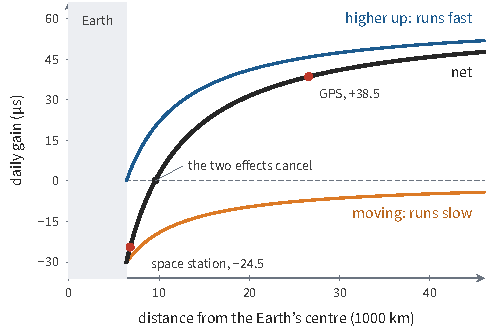
\includegraphics{ch01-clock-offsets}
\caption{How much a clock in a circular orbit gains per day over a clock on
the ground. Height makes the orbiting clock run fast (blue); motion makes it
run slow (orange). You will derive all three curves in \cref{ch:geometry}.
The Earth's rotation, which changes the numbers slightly, is ignored.}
\label{fig:clock-offsets}
\end{figure}

For the navigation satellites the net gain is about 38 microseconds per day.
Left uncorrected, it would spoil positions quickly: light travels
\SI{11}{\kilo\metre} in 38 microseconds, so the ranging error would grow by
about that much every day. The designers of the system corrected for it
before launch, by setting each satellite clock to tick slow by
$4.465$ parts in $10^{10}$ so that, once in orbit, it keeps pace with clocks
on the ground.

Navigation engineers work \emph{within} a geometry that nature has fixed. The
rates of clocks at different heights are set by the mass of the Earth, and the
engineers' job is to measure those rates and correct for them. Spacetime
engineering asks the reverse question. Suppose we could choose the geometry.
What pattern of clock rates, distances and light paths would we want? What
would such a spacetime do to travellers, to light and to ordinary matter? And
what would it take to produce it?

\begin{revisited}{The satellite's clock}
The satellite clock is ahead, by about 38 microseconds a day. At the
satellites' height, the gain from being higher (about 46 microseconds a day)
beats the loss from moving (about 7). The space station is barely higher than
the ground, about \SI{420}{\kilo\metre} up, but moves at
\SI{7.7}{\kilo\metre\per\second}; there the loss wins, and the station's clock
falls behind the ground by about 25 microseconds a day. Astronauts on the
station age slightly less than the rest of us.
\end{revisited}

% ===========================================================================
\section{How hard is it to bend spacetime?}\label{sec:stiff}

\begin{thought}{Denting time in the laboratory}
Popular pictures show gravity as a heavy ball denting a stretched rubber
sheet. Try making a dent yourself. Cast a ball one metre across from osmium,
the densest metal known: about twelve tonnes of it. Set one of today's best
atomic clocks against its surface, and an identical clock at the far end of
the laboratory, well away from it. Such clocks keep time to better than one
part in $10^{18}$. Will they detect the dent the ball makes in the rate of
time?
\end{thought}

Special relativity teaches that space and time are not separate. Observers in
relative motion disagree about lengths and durations, but they agree on the
speed of light and on a combination of time and distance called the
\emph{interval} between two events. Space and time together form a
four-dimensional \emph{spacetime}, and the interval plays the role in it that
distance plays in ordinary geometry.

General relativity takes one step further: the geometry of spacetime can be
curved, and gravity \emph{is} that curvature. An apple falls because it
follows the straightest possible path through a curved spacetime, and clocks
at different heights tick at different rates because the geometry of time
itself varies from place to place. John Wheeler summed up the theory in one
sentence: spacetime tells matter how to move, and matter tells spacetime how
to curve.

The rule for the second half of that sentence is \emph{Einstein's equation}.
In words, it says
\begin{equation}
  \begin{pmatrix}\text{curvature}\\ \text{of spacetime}\end{pmatrix}
  = \frac{8\pi G}{c^{4}}
  \begin{pmatrix}\text{energy, momentum,}\\ \text{pressure and stress}\\
  \text{of matter}\end{pmatrix}.
  \label{eq:einstein-words}
\end{equation}
The left side is built from the geometry. The right side describes
everything that has energy: matter, light and fields, and even the pressure
and tension inside a material. \Cref{ch:matter-geometry} turns both sides into
precise mathematical objects.

The constant in front, $8\pi G/c^{4}$, sets the scale of the whole subject.
Its size is fixed by
\begin{equation}
  \frac{c^{4}}{G} \approx \SI{1.2e44}{\newton},
  \label{eq:stiffness}
\end{equation}
a force, and an enormous one. Read \cref{eq:einstein-words} as a rule for
estimates: to curve spacetime so that its radius of curvature is about $L$,
matter must supply energy densities or stresses of order
$c^{4}/(8\pi G L^{2})$. For $L = \SI{1}{\metre}$ that is about
\SI{5e42}{\pascal}, more than thirty orders of magnitude beyond the breaking
strength of the strongest materials known. Spacetime is extraordinarily stiff.
That single number explains why the geometry around you is so nearly flat, and
it is the first reason spacetime engineering is hard.

A compact mass $M$ slows clocks near it by a fraction that, at a distance $r$
where the effect is small, is
\begin{equation}
  \frac{GM}{c^{2}r} = \frac{M}{r}\Big/\frac{c^{2}}{G},
  \qquad
  \frac{c^{2}}{G} \approx \SI{1.35e27}{\kilogram\per\metre}.
  \label{eq:clock-slowing}
\end{equation}
The ratio $c^{2}/G$ is the stiffness again, expressed as a mass per unit
length. A mass bends time appreciably only when the mass per unit distance
approaches that value.

\begin{example}[label=ex:earth-dent]{How far does the Earth bend time?}
Use \cref{eq:clock-slowing} to find how much slower a clock on the Earth's
surface runs than a clock far out in space. The Earth has mass
$M = \SI{5.97e24}{\kilogram}$ and radius $R = \SI{6.37e6}{\metre}$.

\solution The mass per unit distance is
$M/R = \SI{9.4e17}{\kilogram\per\metre}$. Dividing by $c^{2}/G$ gives
\begin{equation*}
  \frac{GM}{c^{2}R} = \frac{\SI{9.4e17}{}}{\SI{1.35e27}{}} = 7.0\times10^{-10}.
\end{equation*}
A clock on the ground loses 7 parts in $10^{10}$, about 60 microseconds a day,
compared with a clock far away.

\discussion The entire Earth produces less than a part-per-billion effect.
This is the same 60 microseconds a day at which the height curve of
\cref{fig:clock-offsets} levels off far from the Earth.
\end{example}

\begin{checkpoint}[label=chk:sun-ns]
Estimate the fractional slowing of clocks at the surface of the Sun
($M = \SI{2.0e30}{\kilogram}$, $R = \SI{7.0e8}{\metre}$), of a white dwarf of
0.6 solar masses and radius \SI{7000}{\kilo\metre}, and of a neutron star of
1.4 solar masses and radius \SI{12}{\kilo\metre}. For which of them is
\cref{eq:clock-slowing} a safe approximation?
\end{checkpoint}

\begin{revisited}{Denting time in the laboratory}
Not even close. The ball's mass per unit radius is
$\SI{1.2e4}{\kilogram}/\SI{0.5}{\metre} = \SI{2.4e4}{\kilogram\per\metre}$,
and dividing by $c^{2}/G$ in \cref{eq:clock-slowing} gives a slowing of about
$2\times10^{-23}$ at its surface. The clock across the laboratory is slowed by
only a few percent of that, so the difference between the two is still about
$2\times10^{-23}$, tens of thousands of times too small for the best clocks to
see. For the dent to reach one part in $10^{18}$, an osmium ball would have to
be about \SI{240}{\metre} across, some 160 million tonnes. The sheet is that
stiff.
\end{revisited}

% ===========================================================================
\section{Reading the equation backwards}\label{sec:backwards-intro}

\begin{thought}{Can relativity say no?}
A friend hands you a formula for a spacetime in which a ship crosses the
galaxy in an afternoon, and asks whether general relativity allows it.
Einstein's equation is the law that connects geometry to matter. Before you
read on, decide: is there any geometry that Einstein's equation, on its own,
forbids?
\end{thought}

Physicists usually read Einstein's equation from right to left. They describe
the matter first (a star, a galaxy, the contents of the universe) and then
solve for the geometry it produces. This is how the geometry around the Sun
was found, and the geometry of black holes and of the expanding universe. It
is hard work: the equation is a set of coupled, nonlinear partial differential
equations, and only highly symmetric problems can be solved by hand.

A spacetime engineer reads the equation from left to right. Start by deciding
what you want the spacetime to do: carry a traveller quickly between two
places, keep the traveller's clock in step with clocks at home, spare the
traveller from tidal stretching. Write down a geometry that does those things.
Then compute its curvature and read off from \cref{eq:einstein-words} the
matter that would have to be present to produce it. We call that matter the
\emph{demanded} matter of the geometry. In this direction the mathematics is
straightforward: computing curvature from a given geometry takes only
differentiation.

Michael Morris and Kip Thorne introduced this way of working in 1988, in a
paper written for students, to design wormholes a person could travel
through. They first listed the properties a traveller would need, then chose
a geometry with those properties, and only then asked what matter it would
require. The method is now called \emph{metric engineering}, because a
geometry is specified by its \emph{metric}, the object you will meet in
\cref{ch:geometry}.

The catch comes at the last step. Einstein's equation always returns an
answer, and nothing guarantees that the matter it names exists. The demand
might call for negative energy densities, or tensions far beyond any
material's strength, or both. The real work of spacetime engineering begins
there, and it runs as a loop (\cref{fig:design-loop}): test the demand
against everything known about matter, and revise the geometry until the
demand is one that nature might meet.

\begin{figure*}[tb]
\centering
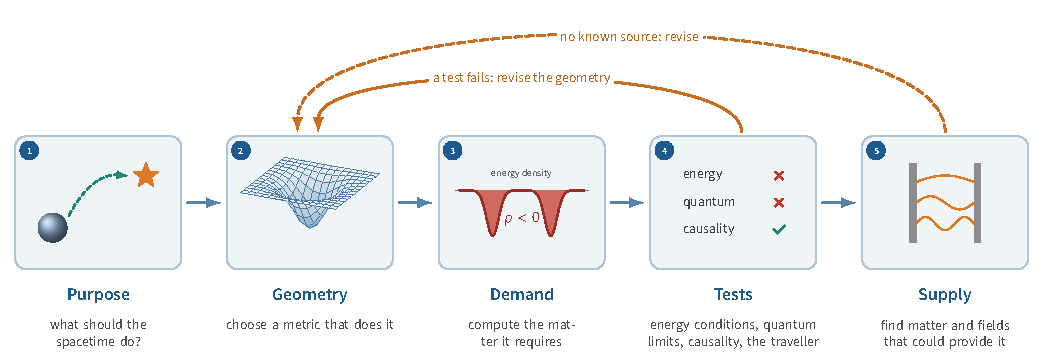
\includegraphics{ch01-design-loop}
\caption{The design loop of spacetime engineering. A geometry is chosen for
what it does, and the matter it demands is computed and tested. When a test
fails, or when no known matter or field could supply the demand, the geometry
is revised. Most of this book teaches the steps inside this loop.}
\label{fig:design-loop}
\end{figure*}

The loop can also be entered from the other side. Some recent work starts
from matter with sensible properties, such as a shell of ordinary material,
solves for the geometry it produces, and then asks what that geometry can do
for a traveller. Both directions appear in this book. The geometry-first
direction is the more common, and it shows most clearly what a design costs.

\begin{checkpoint}[label=chk:division]
Team~A writes down a geometry that carries a ship to a nearby star in a week,
and computes the matter it demands. Team~B takes a moving shell of ordinary
steel and solves Einstein's equation for the geometry it produces. What is
each team sure of, and what must each still find out?
\end{checkpoint}

\begin{revisited}{Can relativity say no?}
Einstein's equation on its own forbids nothing. Read backwards, it assigns
every geometry the matter that would produce it, so it always has an answer.
The question \enquote{does relativity allow this?} therefore becomes
\enquote{does the matter this geometry demands exist, and can it be put in
place?} Your friend's afternoon crossing is possible only if nature can
supply its demand and put it in place, and that is where the physics bites.
\end{revisited}

% ===========================================================================
\section{Three ways to beat a light beam}\label{sec:gallery}

\begin{thought}{The race with a light beam}
A ship and a pulse of light leave the Earth together, bound for a star ten
light-years away. The light travels through ordinary empty space. The ship
reaches the star, turns round, and is home again before the pulse has even
arrived at the star. Yet relativity insists that nothing can overtake a light
signal travelling beside it. How can both be true? Try to invent a way
yourself before reading about the three that physicists have studied.
\end{thought}

\subsection{Tunnels through space}

A wormhole is a tunnel through space: two openings, called mouths, perhaps
light-years apart, joined by a short passage. \Cref{fig:wormhole} shows the
usual way of picturing one. Take a two-dimensional slice through space around
the wormhole and draw it as a curved surface. Far from the wormhole the
surface is flat. Near it, the surface curves into a funnel, narrows to a
smallest circle called the \emph{throat}, and opens out again into a second
region of space.

\begin{figure}[tb]
\centering
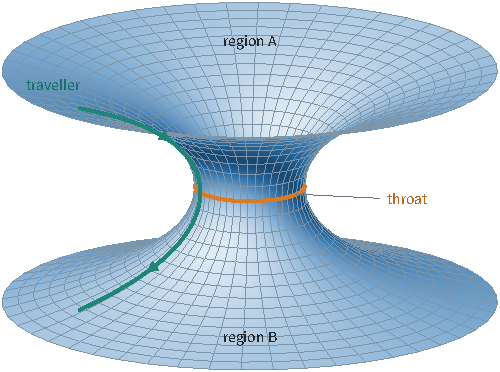
\includegraphics{ch01-wormhole}
\caption{An embedding diagram of a wormhole. A two-dimensional slice of space
is drawn as a surface. Circles around the wormhole shrink toward the throat
and grow again on the far side. A traveller (green) passes from region~A to
region~B through the throat.}
\label{fig:wormhole}
\end{figure}

Wormholes have appeared as solutions of general relativity since the 1930s,
but the early examples could not be crossed: they pinch off faster than
anything can pass through. Morris and Thorne asked what a wormhole would need
to be \emph{traversable}: no horizon at the throat, tidal forces a person
could survive, and a crossing that takes a reasonable time. They found
geometries that meet all these requirements, and then computed what those
geometries demand.

\begin{history}{a novel and a wormhole}
Morris and Thorne took up traversable wormholes after the astronomer Carl
Sagan sent Thorne the draft of his novel \emph{Contact} in 1985 and asked for
help making its physics as accurate as possible. Sagan revised the novel's
method of travel in the light of their preliminary results. Their paper,
subtitled \enquote{a tool for teaching general relativity}, launched the
modern study of engineered spacetimes.
\end{history}

The difficulty lies at the throat. A bundle of light rays heading into a
wormhole converges as it approaches the throat, and to come out the other side
it must spread apart again: the throat has to act on light as a
\emph{diverging} lens. What kind of matter could do that is the question of
the next topic.

\subsection{Moving space itself}

In 1994 Miguel Alcubierre took a different approach. Instead of joining two
distant places by a tunnel, his design moves a region of space itself. Space
contracts in front of a bubble and expands behind it
(\cref{fig:warp}a), and a region of flat spacetime inside the bubble is
carried along. A ship inside that region does not move through its
surroundings at all; it floats in free fall while the bubble carries it.

\begin{figure*}[tb]
\centering
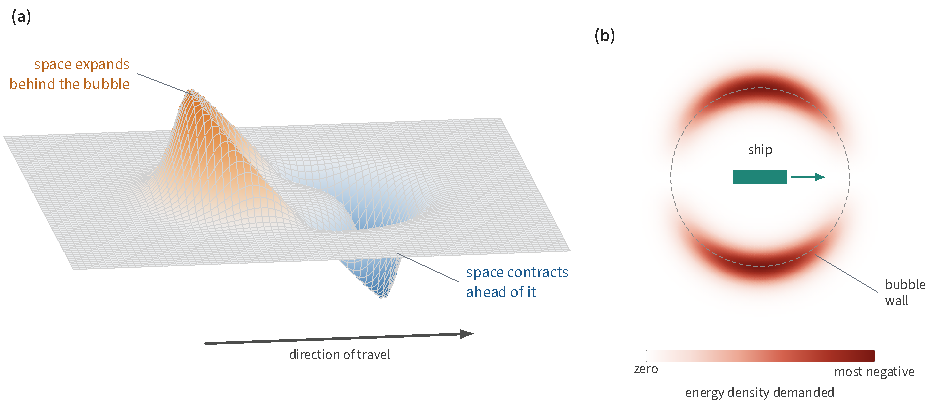
\includegraphics{ch01-warp}
\caption{Alcubierre's warp bubble, in a plane containing the direction of
travel. (a)~The rate at which the volume of space grows (up, orange) or
shrinks (down, blue): space contracts ahead of the bubble and expands behind
it. (b)~The energy density measured by observers carried along by the flow of
space, who far from the bubble are at rest relative to the stars: negative
everywhere it is not zero, and concentrated in a ring around the bubble's
wall.}
\label{fig:warp}
\end{figure*}

Alcubierre's bubble has striking properties. Nothing inside it ever moves
faster than light relative to its own surroundings, yet the bubble as a whole
can move at any speed relative to distant stars. The ship feels no
acceleration, and its clock ticks at the same rate as clocks far away, so the
travellers age exactly as much during the trip as the people they left
behind. José Natário later showed that the expansion and contraction are not
essential: a warp drive can carry its passengers with no change of volume at
all. What \emph{is} essential is the demand. Observers carried along by the
flow of space find a negative energy density in the bubble's wall
(\cref{fig:warp}b), much as observers passing quickly through a wormhole's
throat would find one there.

\begin{checkpoint}[label=chk:warp-aging]
A crew makes a round trip to a star ten light-years away, once in a warp
bubble that moves at five times the speed of light, and once in a ship that
coasts at 99~percent of the speed of light, whose clocks run sevenfold slow.
For each trip, how much does the crew age, and how long do the people at home
wait?
\end{checkpoint}

\subsection{Building the road on the way out}

Sergei Krasnikov pointed out a problem with building and steering warp
drives, which the end of this chapter takes up. His alternative has the
traveller prepare the route on the way out. A ship travels to a distant star at less than the speed of light, and as
it goes it modifies the spacetime along its path, leaving behind a tube. The
modified geometry inside the tube lets the return trip arrive home shortly
after the departure. Allen Everett and Thomas Roman analysed these tubes
further and showed that two of them, suitably placed, would form a time
machine.

\subsection{What recent work has added}

In 2021 several authors proposed warp drives that appeared to need only
positive energy. Examining them closely, Jessica Santiago, Sebastian Schuster
and Matt Visser showed that the positive energy was measured by one special
family of observers only. Other observers passing through the same bubble
measure negative energy, and every physically reasonable warp drive violates
the conditions that ordinary matter satisfies. The episode taught the field a
lesson you will meet throughout this book: the demand of a geometry must be
checked from the point of view of \emph{every} observer. Current research
includes shells of ordinary matter that carry a flat interior at speeds below
that of light, computer simulations of warp spacetimes, and the search for
fields that could supply negative energy.

\begin{revisited}{The race with a light beam}
The light pulse never loses a race run side by side. In every design the ship
stays inside its local \emph{light cone}, the set of directions light can take
from where the ship is, so a light signal sent beside the ship would always
outrun it. What the designs change is the geometry that the ship and the pulse
travel through (\cref{fig:three-ways}). The wormhole shortens the ship's
route, so the pulse through ordinary space runs a longer race. The warp drive
moves the space the ship sits in: inside the bubble the light cones themselves
are tilted toward the ship's destination, and the ship rides inside them. The
Krasnikov tube tips the light cones along a route that the outbound trip has
prepared. There the ship even reaches the star after the pulse does, and yet,
by the clocks at home, it is back before the pulse has reached the star.
\end{revisited}

\begin{figure*}[tb]
\centering
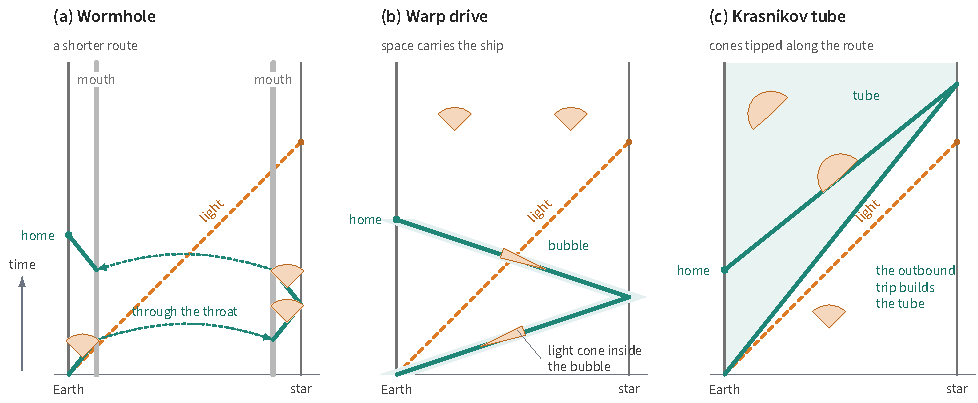
\includegraphics{ch01-three-ways}
\caption{Three ways to reach a star and come home before a light pulse sent
at departure has reached the star, drawn as spacetime diagrams: distance runs
to the right, time runs up, and light travels at \ang{45}. Each wedge shows
the directions light can take from that event; the ship (green) always
travels inside the wedges. (a)~A wormhole shortens the route. (b)~A warp
bubble tilts the light cones inside it. (c)~A Krasnikov tube, laid down by the
outbound trip, tips the cones along the route.}
\label{fig:three-ways}
\end{figure*}

% ===========================================================================
\section{Matter that bends light the wrong way}\label{sec:obstacle}

\begin{thought}{A concave lens made of gravity}
Glass bends light either way: a convex lens focuses a beam, a concave lens
spreads it. Gravity bends light too, and the Sun's gravity focuses starlight
like a weak convex lens. A wormhole throat must spread the light that passes
through it, like a concave lens. Could you build a concave gravitational lens
out of ordinary matter, say from a ring or a hollow shell of very dense
material?
\end{thought}

Gravity bends light toward mass, and the Sun, like every ordinary body, acts
on light as a converging lens (\cref{ex:sun-lens}). Physicists summarize what
ordinary matter can do with a small set of inequalities called
\emph{energy conditions}. The simplest to state is the
\emph{weak energy condition}: every observer, however they move, measures an
energy density that is zero or positive. The most important for this book is
the \emph{null energy condition}, which is weaker still. It concerns light
passing through matter, and it guarantees that the matter's gravity can focus
a bundle of light rays but can never make a shrinking bundle start to grow
again before its rays cross (\cref{fig:focusing}a). Everything you have ever touched satisfies these
conditions, and so do light itself, electric and magnetic fields, and all
ordinary fluids.

\begin{example}[label=ex:sun-lens]{The Sun as a lens}
General relativity predicts that light passing a mass $M$ at distance $b$ is
bent toward it by the angle $4GM/(c^{2}b)$, twice what a Newtonian argument
gives. How strongly does the Sun bend light that grazes its edge, and where
does that light cross the axis on the far side? For the Sun,
$GM/c^{2} = \SI{1.48}{\kilo\metre}$ and $R = \SI{6.96e8}{\metre}$.

\solution For light grazing the edge, $b = R$ and the angle is
\begin{equation*}
  \frac{4 \times \SI{1.48e3}{\metre}}{\SI{6.96e8}{\metre}} = \SI{8.5e-6}{\radian},
\end{equation*}
or 1.75 seconds of arc. A ray bent inward by this small angle reaches the axis
after a distance $R$ divided by the angle, \SI{8.2e13}{\metre}, which is about
550 times the distance from the Earth to the Sun.

\discussion The deflection was first measured during the total solar eclipse
of 1919. Rays passing farther from the Sun are bent less and cross the axis
farther away, so the Sun focuses light along a line that starts some
550~astronomical units out, fourteen times as far as Pluto. The lens is weak,
and it is always a converging one.
\end{example}

\begin{figure}[tb]
\centering
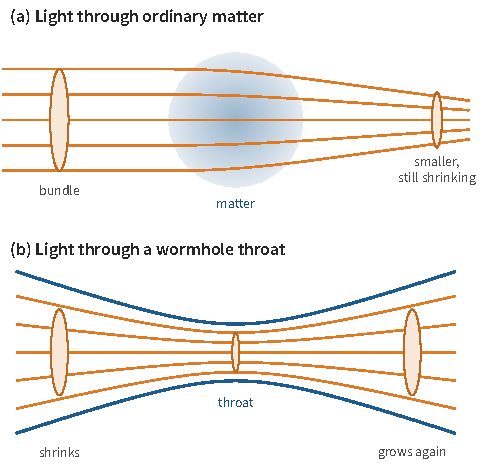
\includegraphics{ch01-focusing}
\caption{(a)~Light passing through ordinary matter is focused: the bundle's
cross-section shrinks, and once it has started to shrink it keeps shrinking
until its rays cross.
(b)~Light passing through a wormhole throat follows the walls: the bundle
shrinks toward the throat and must grow again beyond it.}
\label{fig:focusing}
\end{figure}

The null energy condition is exactly what a shortcut has to violate. A
wormhole throat must make a shrinking bundle of light grow again
(\cref{fig:focusing}b), and a warp bubble's wall must do the same. Morris and
Thorne showed that a throat requires the material there to carry a tension
greater than its energy density, so that observers moving through the throat
close to the speed of light would measure a \emph{negative} energy density.
Matter with such properties is called \emph{exotic}, and you will derive this
requirement yourself in Part~II. In Chapter~5 you will see that it is no
accident. Under quite general
assumptions, any spacetime that lets travellers outrun light through an
otherwise ordinary region of space violates the null energy condition
somewhere.

\begin{keyidea}
Designing a shortcut through spacetime is easy on paper. Supplying the matter
it demands is the hard part: under very general conditions, a shortcut
demands matter that violates the null energy condition, and ordinary matter
never does.
\end{keyidea}

\begin{revisited}{A concave lens made of gravity}
No arrangement of ordinary matter will do. A glass lens spreads light by its
shape: glass slows light, and a concave lens is thicker at its edges than at
its centre. Gravity has no such freedom. The focusing power of matter is set
by the energy density and pressure of the matter that the light passes
through, and for ordinary matter it always focuses. A ring does not help.
Light passing through its middle is tugged one way and then the other, and
along its whole path the tugs cancel exactly, so it emerges undeflected, while
light passing outside the ring is bent inward. Light crossing a shell passes
through its walls, and the walls focus it. The tidal pull of nearby matter can
squeeze a bundle into an ellipse, but it never makes the bundle's area start
to grow. Making a shrinking bundle grow again before its rays cross takes
matter that violates the null energy condition.
\end{revisited}

% ===========================================================================
\section{Negative energy in the laboratory}\label{sec:casimir}

\begin{thought}{A stack of Casimir plates}
Quantum physics allows negative energy densities: between two closely spaced
metal plates, the energy density of the vacuum is lower than that of empty
space. Suppose you want to hold a wormhole's throat open with this negative
energy. Why not simply build an enormous stack of plates?
\end{thought}

In 1948 Hendrik Casimir predicted that two parallel, uncharged metal plates in
vacuum exert a force on each other. The plates restrict which electromagnetic vacuum
fluctuations fit between them, and the energy density between the plates is
lower than that of empty space; measured from empty space, it is negative.
For perfectly conducting plates a distance $d$ apart it is
\begin{equation}
  u = -\frac{\pi^{2}\hbar c}{720\,d^{4}},
  \label{eq:casimir}
\end{equation}
a result you will derive in Chapter~6. Steve Lamoreaux measured the Casimir
force in 1997, and it has since been measured many times. Quantum physics
therefore allows negative energy density.

It allows it only in limited amounts. Lawrence Ford and Thomas Roman showed
that quantum fields obey \emph{quantum inequalities}: the more negative the
energy density in a region, the shorter the time it can last and the smaller
the region it can occupy. Applied to a warp bubble, the inequalities force
the bubble's wall to be extraordinarily thin. Michael Pfenning and Ford
estimated that a bubble \SI{100}{\metre} in radius would then need about
\SI{6e62}{\kilogram} of negative energy for every unit of its speed in units
of $c$, vastly more than the mass of the observable universe. Clever
reshaping of the bubble reduces the requirement dramatically: Chris Van Den
Broeck brought it down to a few solar masses. That is still an astronomical
amount, and his design bends space on scales of about ten Planck lengths, far
below anything that has ever been probed.

\begin{checkpoint}[label=chk:casimir-force]
The energy between the plates is negative. Does that make the plates repel
each other? The energy between them, per unit area of plate, is $u\,d$: as the
plates move closer together, does it rise or fall, which way does the force
point, and how does its strength depend on $d$?
\end{checkpoint}

\begin{revisited}{A stack of Casimir plates}
A stack adds more gaps, but never deeper ones. A gap \SI{1}{\micro\metre} wide
holds about \SI{-4e-4}{\joule\per\cubic\metre}, however many plates surround
it, while a wormhole throat one metre in radius needs a tension exceeding its
energy density by roughly \SI{5e42}{\joule\per\cubic\metre}, some 46 orders of
magnitude more. Because the Casimir energy density grows as $1/d^{4}$,
reaching that value would take plates about \SI{3e-18}{\metre} apart, a few
hundred times smaller than a proton. This is the pattern the quantum
inequalities describe: large negative energy densities are confined to tiny
regions. The plates themselves, besides, carry the positive rest energy of the
metal, about \SI{2e20}{\joule\per\cubic\metre} for aluminium, which outweighs
the gap beside each one by more than twenty orders of magnitude.
\end{revisited}

% ===========================================================================
\section{Cause, effect and control}\label{sec:causality}

\begin{thought}{A message to the front}
You are aboard a warp bubble crossing space at twice the speed of light, and
you decide to stop. The bubble's front wall is only a hundred metres ahead of
you, so you send a radio command forward to shut it down. Does the command
arrive?
\end{thought}

Two further obstacles have nothing to do with the amount of energy. The first
is causality. Relativity allows observers in relative motion to disagree about
which of two distant events happened first, whenever the events are too far
apart for light to connect them. If a signal or a traveller could outrun
light across ordinary space, some observers would therefore see it arrive
before it left. With two faster-than-light links, suitably arranged, a
traveller could return before departing and meet an earlier self. Stephen
Hawking conjectured in 1992 that the laws of physics always prevent this,
a proposal he called the \emph{chronology protection conjecture}. It remains
a conjecture, and a responsible design must show that it creates no such
loops.

The second obstacle is control. A warp bubble is a flow of space. Inside it
the ship floats at rest in its own patch of space; across the bubble's wall
the flow changes to match the space of the distant stars; and light always
moves at the speed of light relative to the space around it. Krasnikov showed
what follows when the bubble outruns light: the crew is cut off from the front
of its own bubble, and can neither build the bubble nor steer it from inside.
Designs that carry travellers faster than light must therefore be laid out in
advance, or driven by something outside the travellers' reach.

\begin{checkpoint}[label=chk:krasnikov-control]
Robot ships leave the Earth at 90~percent of the speed of light for a star ten
light-years away, programmed to shape the wall of a warp bubble along the route
as they pass. Can the crew of a bubble that follows them steer it? How soon,
by the clocks at home, can the first bubble reach the star?
\end{checkpoint}

\begin{revisited}{A message to the front}
It never arrives, however close the wall is. Seen from the bubble, the space outside streams backward
past it at twice the speed of light, and inside the front wall the stream
slows smoothly to zero. Your radio signal moves forward at the speed of light
relative to the space it is in, so somewhere in the wall, where the backward
stream reaches the speed of light, the signal stalls and can advance no
further. The same thing happens to light trying to leave a black hole, and in
\cref{ch:geometry} you will see that this place is a horizon.
\end{revisited}

% ===========================================================================
\section{Where the subject stands}\label{sec:today}

Nobody knows how to build any of the spacetimes in this chapter, and some of
them may be forbidden outright. Spacetime engineering today is a theoretical
discipline, and it earns its place in three ways.

It teaches general relativity. Designing a spacetime forces you to understand
how every piece of its geometry affects clocks, rulers, light and matter. That
was Morris and Thorne's reason for writing their paper, and it is one reason
for this book.

It maps the boundary of the possible. Some of the obstacles above are theorems
with precise assumptions, some are estimates that depend on how a design is
drawn, and some are conjectures. Knowing which is which tells you what would
have to change for a design to become possible, and much of this book is
about learning to tell them apart.

It develops methods that carry over to other problems: how to design under
severe physical constraints, how to check a long calculation, and how to judge
how far a result can be trusted.

The rest of Part~I gives you the tools. \Cref{ch:geometry} develops the
geometry of spacetime: intervals, clocks, the metric, free fall and
curvature. \Cref{ch:matter-geometry} describes matter by its energy, momentum
and stress, states Einstein's equation, and shows how to compute what a
geometry demands. The chapters after them split spacetime into space and time
the way an engineer describes a design, state the energy conditions
precisely, explain what quantum physics allows, and treat causality. Part~II
studies the classic designs in detail. Part~III is about design itself: how
the rate of clocks, the flow of space and the shape of space each affect what
a spacetime demands and what it does to the people inside it. Part~IV asks
what matter and fields could supply a demand, and Part~V takes up dynamics,
the checking of calculations, and the open problems of the field.

This chapter used SI units. From \cref{ch:geometry} on we measure time and
distance in the same units, which sets $c = 1$, and from
\cref{ch:matter-geometry} on we also set $G = 1$. Whenever a number matters,
we convert back to everyday units.

% ===========================================================================
\begin{chaptersummary}
\item Relativity makes identical clocks tick at different rates in different
  places. Satellite navigation works only because its designers correct for
  both the speed and the height of the satellites.
\item Spacetime has a geometry that matter bends; gravity is that bending.
  Einstein's equation links the curvature of spacetime to the energy,
  momentum, pressure and stress of matter.
\item The constant $c^{4}/G \approx \SI{1.2e44}{\newton}$ makes spacetime
  extremely stiff: curving it with a radius of curvature $L$ takes energy
  densities or stresses of order $c^{4}/(8\pi G L^{2})$. A mass $M$ slows
  clocks at distance $r$ by about
  $GM/(c^{2}r)$, which is small unless $M/r$ approaches
  $c^{2}/G \approx \SI{1.35e27}{\kilogram\per\metre}$.
\item Spacetime engineering reads Einstein's equation backwards: choose a
  geometry for what it does, then compute the matter it demands. Every
  geometry has a demand; whether nature can meet it is the real question.
\item The classic designs are traversable wormholes (a shorter route), warp
  drives (space that carries the ship) and Krasnikov tubes (a route prepared
  on the way out). In each, a traveller always moves inside the local light
  cone.
\item All of them demand matter that violates the null energy condition,
  which ordinary matter satisfies. Quantum physics allows negative energy
  density, as the Casimir effect shows, but quantum inequalities limit how
  much, for how long and over how large a region.
\item Faster-than-light designs also face causality (the risk of time
  machines) and control (a bubble moving faster than light cannot be steered
  from inside).
\end{chaptersummary}

\begin{checkanswers}
\item[\ref{chk:sun-ns}] Sun: $GM/(c^{2}R) \approx 2\times10^{-6}$. White dwarf:
  about $1.3\times10^{-4}$. Both are small, so the estimate is safe. Neutron
  star: about $0.17$, not small, so the estimate is rough; the exact result of
  \cref{ch:geometry} is a clock rate of 0.81 of the rate far away. The step
  from star to white dwarf to neutron star is a step in mass per unit radius.
\item[\ref{chk:division}] Team~A is sure its geometry does the job, and it can
  always compute the demand, since that takes only differentiation; it must
  still find out whether matter with that demand can exist and be put in
  place. Team~B is sure its matter exists. It must solve coupled nonlinear
  equations, which is possible by hand only with a great deal of symmetry and
  needs conditions far from the shell as well, and it may find that its
  geometry does nothing useful for a traveller.
\item[\ref{chk:warp-aging}] Warp bubble: the round trip covers 20 light-years at
  five times the speed of light, so it takes 4 years by the clocks at home.
  The crew floats at rest in its own patch of space, and its clocks keep pace
  with those at home, so the crew also ages 4 years. Coasting ship: the trip
  takes $20/0.99 = 20.2$ years at home, while the crew, moving through the
  space around it, ages $20.2/7.09 = 2.85$ years. The fast ship shortens the
  trip only for its crew, who come home to a world 20 years older; the warp
  bubble shortens it for everyone.
\item[\ref{chk:casimir-force}] No: they attract.
  $u\,d = -\pi^{2}\hbar c/(720\,d^{3})$ grows more negative as $d$ shrinks, so
  the energy falls as the plates approach, and the plates move the way that
  lowers it. The force per unit area is the rate at which the energy falls
  with distance, $\pi^{2}\hbar c/(240\,d^{4})$: about \SI{1.3}{\milli\pascal}
  for plates \SI{1}{\micro\metre} apart, rising to a full atmosphere at about
  \SI{11}{\nano\metre}. Laboratory measurements of the attraction agree with
  this prediction.
\item[\ref{chk:krasnikov-control}] No. The robots follow a program fixed
  before they left, and nothing the crew does can reach the parts of the route
  ahead of the bubble. The bubble also cannot outrun the robots that prepare
  its path, so the first trip reaches the star no sooner than they do,
  $10/0.9 = 11.1$ years after they left: later than a light signal would.
  Only later trips gain, once the route is prepared. This is Krasnikov's
  point, and the idea behind his tube.
\end{checkanswers}

\begin{problems}
\item \diff{1} \textbf{Two clocks.} A clock sits at the top of a tower of height
  $h = \SI{100}{\metre}$. Near the Earth's surface, a clock higher by $h$ runs
  faster by the fraction $gh/c^{2}$, where
  $g = \SI{9.8}{\metre\per\second\squared}$. How many nanoseconds does the
  top clock gain over a clock at the base in one year?
\item \diff{1} \textbf{The stiffness of spacetime.} Compute $c^{4}/G$ in newtons
  from $c = \SI{2.998e8}{\metre\per\second}$ and
  $G = \SI{6.674e-11}{\newton\metre\squared\per\kilogram\squared}$. Then
  estimate the stress, in pascals, needed to curve spacetime appreciably over a
  distance of \SI{1}{\kilo\metre}, and compare it with the tensile strength of
  steel, about \SI{e9}{\pascal}.
\item \diff{1} \textbf{A season in orbit.} An astronaut spends six months on the
  space station. Using \cref{fig:clock-offsets}, estimate how much less the
  astronaut ages than someone who stayed on the ground.
\item \diff{2} \textbf{A day of navigation error.} Using the numbers in this
  chapter, find how long it would take an uncorrected navigation-satellite
  clock to drift by the \SI{30}{\nano\second} that corresponds to about
  \SI{10}{\metre} of position error.
\item \diff{2} \textbf{How much is too much?} Express the Pfenning--Ford estimate
  of \SI{6e62}{\kilogram} in solar masses, taking
  $\Msun = \SI{2.0e30}{\kilogram}$. Van Den Broeck's design needs a few solar
  masses. By what factor did reshaping the bubble reduce the requirement?
\item \diff{2} \textbf{Casimir numbers.} Evaluate \cref{eq:casimir} for plates
  \SI{100}{\nano\metre} apart. How thick a layer of this negative energy
  density, spread over the surface of a sphere of radius \SI{1}{\metre}, would
  contain a total negative energy equal to the rest energy of one gram of
  matter?
\item \diff{3} \textbf{Which assumptions?} The quantum inequalities rest on
  assumptions: the kind of quantum field, the flatness of spacetime over the
  sampling time, and the way the energy is averaged. For each, describe how a
  designer might try to take advantage of it, and what you would check to see
  whether the attempt succeeds. Return to your answer after Chapter~6.
\end{problems}

\begin{furtherreading}
\item[\textcite{Ashby2003}] The complete relativistic treatment of satellite
  navigation, including the clock corrections of the first topic.
\item[\textcite{Einstein1916}] Einstein's own presentation of general
  relativity, still readable today.
\item[\textcite{Dyson1920}] The eclipse expedition of 1919 that measured the
  Sun's bending of starlight.
\item[\textcite{Brewer2019}] An atomic clock that keeps time to better than one
  part in $10^{18}$, the precision assumed in the thought experiment on
  denting time.
\item[\textcite{Morris1988a}] The paper that started the field, written for
  students and still one of the best introductions to engineered spacetimes.
\item[\textcite{McMonigal2012,Schuster2023}] Two treatments of metric
  engineering as a method.
\item[\textcite{Alcubierre1994}] The five-page paper that introduced the warp
  drive, readable after \cref{ch:matter-geometry}.
\item[\textcite{Natario2002}] Warp drives without expansion.
\item[\textcite{Krasnikov1998,Everett1997}] Krasnikov's tube, and its
  analysis, including the time machine that two tubes would form.
\item[\textcite{Santiago2022}] Why every physically reasonable warp drive
  violates the energy conditions.
\item[\textcite{Olum1998}] Why travel faster than light through ordinary
  space requires negative energy.
\item[\textcite{Casimir1948,Lamoreaux1997}] The prediction of the Casimir
  effect and its first precise measurement.
\item[\textcite{Ford1995,Ford1997,Pfenning1997}] Quantum inequalities, and what
  they imply for wormholes and warp bubbles.
\item[\textcite{VanDenBroeck1999}] How reshaping a warp bubble reduces its
  energy requirement.
\item[\textcite{Hawking1992}] The chronology protection conjecture.
\item[\textcite{Everett2011}] A book-length, non-technical account of warp
  drives, wormholes and time travel by two researchers who helped shape the
  field.
\item[\textcite{Visser1995b}] The standard monograph on wormholes.
\item[\textcite{Kontou2020}] A modern review of energy conditions in classical
  and quantum physics, useful throughout this book.
\end{furtherreading}

% !TEX root = ../main.tex
\chapteropening{%
A spacetime engineer designs geometries, so we need a precise language for
geometry. This chapter builds it from spacetime diagrams up to curvature.

With it you will be able to compute what a traveller would experience in any
spacetime: the ticking of clocks, the paths of light, the motion of falling
bodies and the stretching forces called tides.}{%
\item draw and read spacetime diagrams, worldlines and light cones;
\item compute the interval between two events and say what can influence
  what;
\item compute the time a clock records along any path;
\item use a metric in any coordinates, and tell a feature of the coordinates
  from a feature of the geometry;
\item compute clock rates in weak gravity and near a black hole, and picture a
  black hole as flowing space;
\item describe free fall as motion along a geodesic, and curvature as the
  source of tides.}
\chapter{The Geometry of Spacetime}\label{ch:geometry}

% ===========================================================================
\section{What every observer agrees on}\label{sec:interval}

\begin{thought}{Has Betelgeuse exploded?}
Betelgeuse, the red supergiant at Orion's shoulder, is roughly 550 light-years
away, and one day it will explode as a supernova. Suppose that, in the frame
in which the Earth and the star are at rest, it explodes at the very moment you
read this sentence. At that moment a ship passes the Earth, heading for
Betelgeuse at half the speed of light. Much later, working back from what they
have seen, the crew concludes that the explosion happened 318 years before
they passed you. Could they have seen it in time to warn you? And how far away
was the star, by their reckoning, when it exploded?
\end{thought}

An \emph{event} is a place at an instant: a firecracker going off at a
particular point and time. We label events with four coordinates, a time $t$
and three positions $x$, $y$, $z$. A particle traces out a continuous sequence
of events called its \emph{worldline}. A \emph{spacetime diagram} plots
worldlines with time running up the page and one direction of space across it
(\cref{fig:spacetime-diagram}). A particle at rest has a vertical worldline; a
moving particle has a tilted one, and the faster it moves the more its
worldline leans over.

\begin{figure}[tb]
\centering
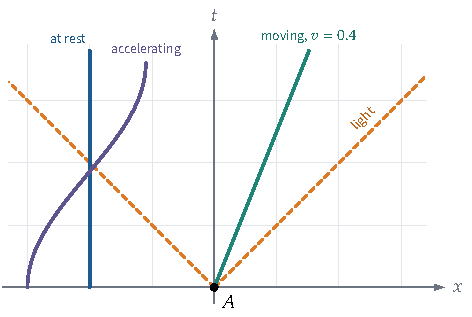
\includegraphics{ch02-spacetime-diagram}
\caption{A spacetime diagram, with time running up the page. A particle at
rest has a vertical worldline and a moving particle a tilted one; a particle
that speeds up and slows down has a curved one. With $c = 1$, light travels
along lines at \ang{45}.}
\label{fig:spacetime-diagram}
\end{figure}

It pays to measure time and distance in the same units. A light-second is the
distance light travels in one second, about \SI{3e8}{\metre}. If we measure
distance in light-seconds and time in seconds, or time in metres (one metre
of time is the time light takes to travel a metre, about
\SI{3.3}{\nano\second}), then the speed of light is exactly $c = 1$ and
velocities become pure numbers: a speed of $0.5$ is half the speed of light.
From here on we use these units, and we restore the factors of $c$ whenever we
need a number in everyday units. Light worldlines then run at \ang{45} on every
spacetime diagram.

In ordinary space, two surveyors who use differently oriented axes disagree
about the coordinates of two points but agree on the distance between them:
$\Delta x^{2} + \Delta y^{2} + \Delta z^{2}$ is the same for both. Special
relativity has an exact analogue. Observers moving relative to one another
disagree about time differences and about distances, yet all of them agree on
the \emph{interval}
\begin{equation}
  \Delta s^{2} = -\Delta t^{2} + \Delta x^{2} + \Delta y^{2} + \Delta z^{2}.
  \label{eq:interval}
\end{equation}
The minus sign in front of the time difference is the whole difference between
the geometry of spacetime and the geometry of space. It sorts pairs of events
into three kinds. The interval is \textbf{timelike} if $\Delta s^{2} < 0$: a
clock can travel from one event to the other at less than the speed of light.
It is \textbf{null}, or lightlike, if $\Delta s^{2} = 0$: a light signal can
travel from one to the other. It is \textbf{spacelike} if
$\Delta s^{2} > 0$: nothing, not even light, can travel from one to the other.

The events that light can reach from an event $A$ form a cone, the
\emph{future light cone} of $A$ (\cref{fig:light-cone}). Events inside it can
be influenced by what happens at $A$; events outside it cannot. The events
from which light can reach $A$ form its past light cone. The light cones of all
events together make up the \emph{causal structure} of spacetime: they tell
you what can affect what. Every question about faster-than-light travel is, at
bottom, a question about light cones.

The interval also settles when the order of two events is shared. For a
timelike or null pair, every observer agrees which came first, since a signal
could pass from one to the other. For a spacelike pair, observers in relative
motion can disagree about the order, and none of them is wrong;
\cref{prob:simultaneity} shows how.

\begin{figure}[tb]
\centering
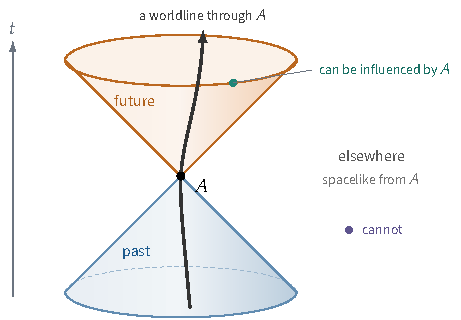
\includegraphics{ch02-light-cone}
\caption{The light cone of an event $A$, with one dimension of space
suppressed. Events inside the future cone can be influenced by $A$, and events
inside the past cone can influence it. Events outside both cones are
spacelike from $A$: no signal connects them to it.}
\label{fig:light-cone}
\end{figure}

\begin{checkpoint}[label=chk:classify]
Event $B$ happens \SI{3}{\second} after event $A$ and 4~light-seconds away
from it. Event $C$ happens \SI{5}{\second} after $A$, at the same place as $B$.
A probe travels from $A$ to $C$ at constant velocity: how fast does it go, and
how much time does its clock record? Could any probe be present at both $A$
and $B$? For an observer who finds $A$ and $B$ simultaneous, how far apart are
they?
\end{checkpoint}

\begin{revisited}{Has Betelgeuse exploded?}
No warning was possible. In the Earth's frame the two events, you reading and
the star exploding, are 550 light-years apart with no time between them, so
$\Delta s^{2} = (\text{550 light-years})^{2}$: a spacelike interval. The crew
must find the same interval. With $\Delta t' = 318$ years,
$\Delta x'^{2} = 550^{2} + 318^{2}$ in light-years squared, so by their
reckoning the star was 635 light-years away when it exploded, not the 476 that
length contraction gives for its distance as they pass you. Its light needs
635 years to reach them and has had only 318, so it is still some 318
light-years away when they pass you. The crew places the explosion in the
past, you place it in the present, and an observer flying away from the star
would place it in the future (\cref{prob:simultaneity}). For events with a
spacelike interval the order in time is not the same for everyone, and no
observer's version is privileged; yet no one can use the difference to send a
signal.
\end{revisited}

% ===========================================================================
\section{The time a clock keeps}\label{sec:proper-time}

\begin{thought}{The twins}
Twins say goodbye on Earth. One boards a ship to Proxima Centauri, 4.24
light-years away, travelling at 80 percent of the speed of light; she turns
round in a single day and comes straight back at the same speed. On each leg
of the trip, each twin measures the other's clock running slow, so the
situation looks symmetric. When they meet again, who is younger, and by how
much? A common answer blames the turnaround, since only the traveller
accelerates. If that were right, how would the answer change for a star ten
times as far away, with the same one-day turnaround?
\end{thought}

A clock carried along a worldline measures the \emph{proper time} $\tau$ along
it. For a clock at rest, proper time is just coordinate time. For a moving
clock the interval does the bookkeeping. Along a short piece of a timelike
worldline the interval is negative, and the clock records
\begin{equation}
  \dd\tau^{2} = -\dd s^{2} = \dd t^{2} - \dd x^{2} - \dd y^{2} - \dd z^{2}.
  \label{eq:proper-time}
\end{equation}
Dividing by $\dd t^{2}$ gives $\dd\tau/\dd t = \sqrt{1 - v^{2}}$, where $v$ is
the clock's speed, and the proper time along a whole worldline is the sum of
the pieces:
\begin{equation}
  \tau = \int \sqrt{1 - v(t)^{2}}\;\dd t .
  \label{eq:proper-time-integral}
\end{equation}
This is the time dilation of special relativity written as a geometric length:
proper time is to a worldline what length is to a curve in space.

\begin{example}[label=ex:muon]{Muons from the sky}
Cosmic rays striking the upper atmosphere create muons about
\SI{15}{\kilo\metre} up, and many of them head for the ground at
$v = 0.9995$. A muon at rest decays after \SI{2.2}{\micro\second} on average.
How much time passes on a muon's own clock during the trip down?

\solution In the Earth's frame the trip takes
\begin{equation*}
  \Delta t = \frac{\SI{15}{\kilo\metre}}{0.9995\,c} = \SI{50.1}{\micro\second}.
\end{equation*}
The muon moves at constant speed, so \cref{eq:proper-time-integral} gives
\begin{equation*}
  \Delta\tau = \sqrt{1 - 0.9995^{2}}\;\Delta t = 0.0316 \times \SI{50.1}{\micro\second}
  = \SI{1.58}{\micro\second}.
\end{equation*}

\discussion The trip takes less than one mean lifetime on the muon's clock, so
about half the muons survive it. Measured in Earth time the trip lasts 23
lifetimes, and without time dilation only about one muon in eight billion
would reach the ground. Detectors on the ground see the larger number.
\end{example}

\begin{keyidea}
Between two events, the straight worldline of a freely moving clock records
the longest proper time. Every other worldline between the same two events,
however it bends, records less.
\end{keyidea}

\begin{checkpoint}[label=chk:zigzag]
Two events happen at the same place, ten years apart. Describe a worldline
between them along which a clock records as little time as you like. Is there
a worldline of \emph{least} proper time?
\end{checkpoint}

\begin{revisited}{The twins}
The traveller is younger, by 4.24 years. In the Earth's frame the round trip
covers 8.48 light-years at speed 0.8 and takes 10.6 years; on her clock it
takes $0.6 \times 10.6 = 6.36$ years. For a star ten times as far away the gap
grows tenfold, to 42.4 years, although the turnaround is unchanged: the
ageing builds up along the whole trip, not at the corner. Between the same
two events, the traveller's bent worldline is shorter than the Earth twin's
straight one (\cref{fig:twins}). The symmetry is only apparent, and the twins
can check it by sending each other a signal every year. Each receives the
other's signals at a third of the rate they are sent while the two move
apart, and at three times the rate while they approach. The traveller
switches from one to the other at her turnaround, halfway through her trip,
and receives $1.06 + 9.54 = 10.6$ years' worth of Earth's signals. The Earth
twin receives slow signals until the light from the turnaround arrives, 9.54
years after the start, and fast ones only for the last 1.06 years:
$3.18 + 3.18 = 6.36$ years' worth.
\end{revisited}

\begin{figure}[tb]
\centering
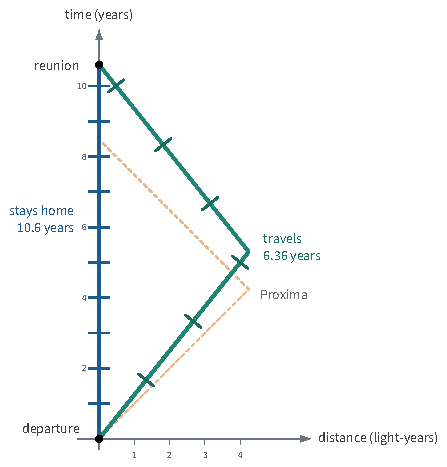
\includegraphics{ch02-twins}
\caption{The twins' worldlines. Each tick marks one year on that twin's own
clock. The straight worldline of the twin who stays home collects 10.6 ticks;
the bent worldline of the traveller collects 6.36.}
\label{fig:twins}
\end{figure}

% ===========================================================================
\section{The metric: measuring with any grid}\label{sec:metric}

\begin{thought}{A current faster than light}
In \cref{ch:what-is}, a radio command sent forward inside a warp bubble
stalled in the bubble's wall, where space streamed backward past the ship at
the speed of light. Suppose instead that space streams past a grid of
coordinates at twice the speed of light, at the same rate everywhere. Two
probes drift with the stream, one light-second apart, and the downstream probe
radios the upstream one. Does the message ever arrive?
\end{thought}

\Cref{eq:interval} holds for inertial observers using Cartesian coordinates. We
need a version that works in any coordinates, and later in curved spacetime.
The idea is to give the interval between \emph{neighbouring} events as a
formula in whatever coordinates we are using.

We label the four coordinates with an index that runs from 0 to 3:
$x^{0} = t$, $x^{1} = x$, $x^{2} = y$, $x^{3} = z$. The raised index is a
label, not a power, and Greek letters $\mu, \nu, \dots$ stand for any of the
four values. The interval between neighbouring events is then
\begin{equation}
  \dd s^{2} = g_{\mu\nu}\,\dd x^{\mu}\,\dd x^{\nu},
  \label{eq:metric}
\end{equation}
where we use the \emph{summation convention}: an index that appears once up and
once down in a term is summed from 0 to 3, so the right side stands for
$\sum_{\mu}\sum_{\nu} g_{\mu\nu}\,\dd x^{\mu}\dd x^{\nu}$. The sixteen numbers
$g_{\mu\nu}$ form a symmetric $4\times4$ matrix called the \emph{metric}. For
flat spacetime in Cartesian coordinates, comparison with \cref{eq:interval}
gives the Minkowski metric
\begin{equation*}
  g_{\mu\nu} = \eta_{\mu\nu} =
  \begin{pmatrix} -1 & 0 & 0 & 0\\ 0 & 1 & 0 & 0\\ 0 & 0 & 1 & 0\\ 0 & 0 & 0 & 1\end{pmatrix}.
\end{equation*}

The same flat spacetime looks different in other coordinates. In spherical
coordinates the interval reads
\begin{equation}
  \dd s^{2} = -\dd t^{2} + \dd r^{2} + r^{2}\,\dd\Omega^{2},
  \label{eq:flat-spherical}
\end{equation}
with $\dd\Omega^{2} = \dd\theta^{2} + \sin^{2}\theta\,\dd\phi^{2}$. The metric
components now depend on position, yet nothing physical has changed.
Coordinates are labels we attach to events, and much of the skill of working
with metrics lies in telling which features of a metric belong to the labels
and which belong to the geometry. The next example shows how dramatic a pure
effect of the labels can look.

\begin{example}[label=ex:flow]{Flowing coordinates}
Consider the metric
\begin{equation}
  \dd s^{2} = -\dd t^{2} + \bigl(\dd x - v_{0}\,\dd t\bigr)^{2} + \dd y^{2} + \dd z^{2},
  \label{eq:flow-metric}
\end{equation}
with $v_{0}$ a constant. Find the coordinate speed $\dd x/\dd t$ of light moving
along $x$, and show that this metric describes flat spacetime.

\solution Light has $\dd s^{2} = 0$. Along $x$ we set $\dd y = \dd z = 0$ and
find $(\dd x - v_{0}\,\dd t)^{2} = \dd t^{2}$, so $\dd x - v_{0}\,\dd t = \pm\dd t$
and
\begin{equation*}
  \frac{\dd x}{\dd t} = v_{0} \pm 1.
\end{equation*}
Now change coordinates to $x' = x - v_{0}t$, keeping $t$, $y$ and $z$. Then
$\dd x' = \dd x - v_{0}\,\dd t$, and the metric becomes
$\dd s^{2} = -\dd t^{2} + \dd x'^{2} + \dd y^{2} + \dd z^{2}$, the Minkowski
metric.

\discussion This is flat spacetime described with a grid whose points slide
along $-x$ at speed $v_{0}$ past inertial observers. The warp drives of
\cref{ch:what-is} have metrics of exactly this form, with $v_{0}$ replaced by a
function that varies from place to place, and then the effect is no longer
only a matter of labels.
\end{example}

The form \cref{eq:flow-metric} gives us a picture that runs through this book:
space \emph{flowing} past a grid of coordinates. Observers carried along by the
flow feel no force. The flow speed can take any value. Where it varies from
place to place the geometry may be genuinely curved, though not always: a flow
that rotates rigidly, for instance, is still flat spacetime in rotating
coordinates, and only a calculation of curvature settles the question.

The tangent to a worldline, measured per unit proper time, is the
\emph{four-velocity} $u^{\mu} = \dd x^{\mu}/\dd\tau$. Dividing \cref{eq:metric}
by $\dd\tau^{2} = -\dd s^{2}$ gives its normalization,
\begin{equation}
  g_{\mu\nu}\,u^{\mu}u^{\nu} = -1.
  \label{eq:four-velocity}
\end{equation}
For a clock at rest in flat spacetime, $u^{\mu} = (1,0,0,0)$; for a clock moving
at speed $v$ along $x$, $u^{\mu} = \gamma\,(1, v, 0, 0)$ with
$\gamma = 1/\sqrt{1-v^{2}}$. In \cref{ch:matter-geometry} four-velocities tell
us what an observer measures.

\begin{checkpoint}[label=chk:grid-clock]
In the flowing coordinates of \cref{ex:flow} with $v_{0} = 0.6$, a clock rides
with one grid point, at fixed $x$. How much time does it record while the
coordinate time $t$ advances by ten years? Compare with the time dilation of a
clock moving at speed $0.6$.
\end{checkpoint}

\begin{revisited}{A current faster than light}
It arrives after one second, exactly as if there were no stream at all. A
stream that is the same everywhere is flat spacetime described with sliding
coordinates: it is \cref{eq:flow-metric} with $v_{0} = 2$, and in the
coordinates $x' = x - v_{0}t$ of \cref{ex:flow} the metric is Minkowski and
both probes sit at rest. In the grid coordinates the numbers look alarming.
The probes move at $\dd x/\dd t = 2$, and the message, sent upstream, moves at
$v_{0} - 1 = +1$, carried downstream by the stream; yet the upstream probe
gains on it and meets it one second later. What stalled the command in the
warp bubble is something no change of coordinates removes: a stream that
changes, across the wall, from nothing to faster than light. A horizon needs
flow that reaches the speed of light next to slower flow, where an observer
can hold position against it, as in the river of space two topics ahead.
\end{revisited}

% ===========================================================================
\section{Clocks in a gravitational field}\label{sec:clocks}

\begin{thought}{Light climbing a tower}
\Cref{ch:what-is} told you that a clock at the top of a tower runs fast
compared with one at its foot, by the fraction $gh/c^{2}$. A laser at the foot
shines a steady beam up to a detector at the top. Each photon carries the
energy $E = hf$, where $f$ is the light's frequency and $h$ is Planck's
constant, and energy has weight, so each photon loses the fraction $gh/c^{2}$
of its energy on the way up. Someone reasons that the detector must find the
frequency lower by $2gh/c^{2}$ in all: once because the light arrives with
less energy, and again because the detector's clock runs fast. Is that right?
\end{thought}

In curved spacetime no choice of coordinates puts the metric into the
Minkowski form everywhere at once. The metric still gives the interval between
neighbouring events through \cref{eq:metric}, and the proper time along a
worldline is still $\tau = \int\sqrt{-\dd s^{2}}$. Everything we did above
carries over; only the metric changes.

Around a planet or a star the gravitational field is weak and the metric is
very close to Minkowski. To an excellent approximation,
\begin{equation}
  \begin{split}
  \dd s^{2} = {}&-(1 + 2\Phi)\,\dd t^{2}\\
  &+ (1 - 2\Phi)\bigl(\dd x^{2} + \dd y^{2} + \dd z^{2}\bigr),
  \end{split}
  \label{eq:weak-field}
\end{equation}
where $\Phi$ is the Newtonian gravitational potential divided by $c^{2}$. For a
spherical mass $M$, $\Phi = -GM/(c^{2}r)$, small and negative:
$\Phi \approx -7\times10^{-10}$ at the Earth's surface, as in
\cref{ex:earth-dent}. The approximation holds wherever $|\Phi| \ll 1$.

A clock moving slowly at speed $v$ through this spacetime records, from
\cref{eq:weak-field},
\begin{equation}
  \begin{split}
  \frac{\dd\tau}{\dd t} &= \sqrt{1 + 2\Phi - (1 - 2\Phi)\,v^{2}}\\
  &\approx 1 + \Phi - \tfrac{1}{2}v^{2},
  \end{split}
  \label{eq:clock-rate}
\end{equation}
keeping only the leading terms in the small quantities $\Phi$ and $v^{2}$. The
two corrections have a clear meaning: a clock deeper in the potential (more
negative $\Phi$) runs slower, and a moving clock runs slower.

The same clock rates set what a receiver finds in a signal. The metric
\cref{eq:weak-field} does not change with $t$, so every wave crest sent from
one place to another takes the same coordinate time for the trip: crests that
leave a transmitter a coordinate interval $\Delta t$ apart arrive $\Delta t$
apart. Each clock converts $\Delta t$ into its own time at its own rate. A
receiver higher up, where clocks run faster, counts more of its own time
between crests than the transmitter did, and so measures a lower frequency,
lower by the fractional difference in potential, $\Delta\Phi$. This is the
\emph{gravitational redshift}. Near the ground $\Delta\Phi = gh/c^{2}$ for a
height difference $h$. In 1960 Robert Pound and Glen Rebka measured it with
gamma rays sent up and down a tower \SI{22.6}{\metre} tall at Harvard, where the
shift is only $2.5\times10^{-15}$, and their result agreed with the prediction
to within ten percent. Today's optical clocks detect the change in rate when
one of them is raised by just \SI{33}{\centi\metre}, a shift of four parts in
$10^{17}$.

\begin{example}[label=ex:gps, unbreakable]{Clocks on the ground and in orbit}
Navigation satellites orbit at a radius
$r_{\mathrm{sat}} = \SI{26560}{\kilo\metre}$. Take
$GM = \SI{3.986e14}{\metre\cubed\per\second\squared}$ and
$R = \SI{6371}{\kilo\metre}$ for the Earth, and ignore its rotation. How much
does a satellite clock gain each day over a clock on the ground?

\solution The ground clock is at rest at $r = R$, so its rate is $1 + \Phi(R)$.
The satellite clock moves on a circular orbit at speed
$v = \sqrt{GM/r_{\mathrm{sat}}} = \SI{3.87}{\kilo\metre\per\second}$. In SI
units the difference in rates is
\begin{equation*}
  \frac{GM}{c^{2}}\left(\frac{1}{R} - \frac{1}{r_{\mathrm{sat}}}\right)
  - \frac{v^{2}}{2c^{2}},
\end{equation*}
a gain from height of $5.29\times10^{-10}$ and a loss from speed of
$8.35\times10^{-11}$. Over one day, \SI{86400}{\second}, the satellite clock
gains \SI{45.7}{\micro\second} from its height and loses
\SI{7.2}{\micro\second} from its speed, a net gain of
\SI{38.5}{\micro\second}.

\discussion These are the numbers behind \cref{fig:clock-offsets}. Repeating
the calculation for every orbital radius draws the three curves of that
figure (\cref{prob:gps-curves}).
\end{example}

For a non-rotating mass $M$, and with no weak-field approximation at all, the
geometry outside the mass is the \emph{Schwarzschild metric},
\begin{equation}
  \begin{split}
  \dd s^{2} = {}&-\Bigl(1 - \frac{r_{\mathrm{s}}}{r}\Bigr)\dd t^{2}
  + \frac{\dd r^{2}}{1 - r_{\mathrm{s}}/r}\\
  &+ r^{2}\,\dd\Omega^{2},
  \end{split}
  \label{eq:schwarzschild}
\end{equation}
with $r_{\mathrm{s}} = 2GM/c^{2}$. Here $r$ is defined so that a sphere at
radius $r$ has area $4\pi r^{2}$. A clock held at fixed $r$ records
$\dd\tau/\dd t = \sqrt{1 - r_{\mathrm{s}}/r}$ relative to a clock far away. For
the Sun $r_{\mathrm{s}} \approx \SI{2.95}{\kilo\metre}$, so the effect at its
surface is tiny, but a clock on the surface of a neutron star runs at about
0.81 of the rate of a distant clock (\cref{prob:neutron-star}).

At $r = r_{\mathrm{s}}$ the clock rate would fall to zero: no clock can be held
at rest there. The sphere $r = r_{\mathrm{s}}$ is the \emph{event horizon} of a
black hole. The metric \cref{eq:schwarzschild} also misbehaves there, where
$g_{rr}$ becomes infinite, but that part is an artefact of the labels, as the
next topic shows.

\begin{checkpoint}[label=chk:earth-centre]
A clock sits in a small cavity at the centre of the Earth. It feels no pull at
all, just like a clock far out in space. Does it keep the same rate as the
distant clock? Is it faster or slower than a clock on the Earth's surface?
\end{checkpoint}

\begin{revisited}{Light climbing a tower}
No: the frequency is lower by $gh/c^{2}$, once. The geometry does not change
with time, so crests reach the top exactly as often as they leave the bottom,
counted in the coordinate time $t$. The only difference between the two ends
is the rate of their clocks. The top clock runs faster, so it counts a longer
time between crests and reports a frequency lower by $gh/c^{2}$, and with
$E = hf$ that lower frequency \emph{is} the lost energy. The energy loss and
the fast clock are one effect described twice, and adding them counts it
twice. Pound and Rebka measured $1.05 \pm 0.10$ times the prediction, which
rules out the doubled value.
\end{revisited}

% ===========================================================================
\section{Space as a flowing river}\label{sec:river}

\begin{thought}{Standing still in the river}
A probe hangs on a long cable at twice the horizon radius of a black hole,
$r = 2r_{\mathrm{s}}$. Its clock runs at $\sqrt{1 - r_{\mathrm{s}}/r} = 0.71$ of
the rate of clocks far away. A second probe, dropped from rest far away, falls
past it at 71~percent of the speed of light. Moving clocks run slow; but which
of these two probes is moving? Is it a coincidence that the two numbers match?
\end{thought}

Introduce a new time coordinate $T$: the time on the clocks of observers who
fall inward from rest far away. In these coordinates the Schwarzschild geometry
takes the Painlevé--Gullstrand form,
\begin{equation}
  \dd s^{2} = -\dd T^{2} + \Bigl(\dd r + \sqrt{\tfrac{r_{\mathrm{s}}}{r}}\;\dd T\Bigr)^{2}
  + r^{2}\,\dd\Omega^{2}.
  \label{eq:river}
\end{equation}
Compare it with \cref{eq:flow-metric}. It has the same form, with space flowing
\emph{inward} at the speed $\sqrt{r_{\mathrm{s}}/r}$, which grows as $r$ shrinks
(\cref{fig:river}). Nothing is singular at $r = r_{\mathrm{s}}$ any more. Radial
light obeys $\dd s^{2} = 0$, which gives
\begin{equation}
  \frac{\dd r}{\dd T} = -\sqrt{\frac{r_{\mathrm{s}}}{r}} \pm 1 :
  \label{eq:river-light}
\end{equation}
light always moves at speed 1 relative to the space around it, and the space
carries it inward. Like a fish in a river that runs ever faster toward a
waterfall, outgoing light makes headway only where the flow is slower than its
own speed. At $r = r_{\mathrm{s}}$ the flow reaches the speed of light, and
inside that sphere even outgoing light is swept inward: the sphere is the
horizon. This picture, developed by Andrew Hamilton and Jason Lisle as the
\emph{river model} of black holes, will be our main intuition for geometries
whose space flows.

\begin{figure}[tb]
\centering
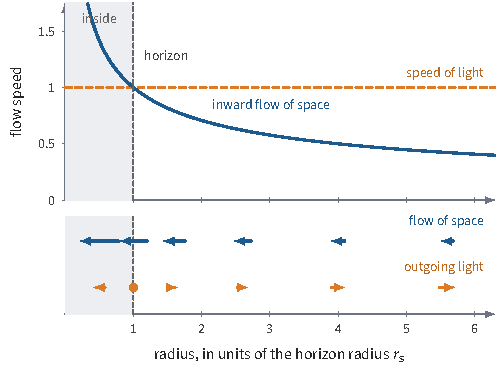
\includegraphics{ch02-river}
\caption{The Schwarzschild geometry pictured as space flowing inward
(\cref{eq:river}). Top: the inward flow speed $\sqrt{r_{\mathrm{s}}/r}$
(blue) reaches the speed of light (dashed) at the horizon. Bottom: the flow
drawn to scale (blue), and the net speed of outgoing light (orange), which
falls to zero at the horizon and turns inward inside it.}
\label{fig:river}
\end{figure}

\begin{example}[label=ex:earth-river]{The river at the Earth's surface}
In SI units the flow speed is $v = c\sqrt{r_{\mathrm{s}}/r} = \sqrt{2GM/r}$. How
fast does space flow inward at the surface of the Earth?

\solution With $GM = \SI{3.986e14}{\metre\cubed\per\second\squared}$ and
$r = \SI{6.371e6}{\metre}$,
\begin{equation*}
  v = \sqrt{\frac{2 \times 3.986\times10^{14}}{6.371\times10^{6}}}\ \si{\metre\per\second}
  = \SI{11.2}{\kilo\metre\per\second}.
\end{equation*}

\discussion This is the Earth's escape speed. The river of space flows at the
Newtonian escape speed everywhere, which is why an observer falling from rest
far away, carried along by the river, arrives at each radius with exactly that
speed.
\end{example}

\begin{history}{dark stars}
In a paper read to the Royal Society in 1783, John Michell asked what gravity
does to light leaving a star. Treating light as particles obeying Newton's
laws, he found that a star with the Sun's density and 500 times its radius
would have an escape speed greater than the speed of light, so its light
could never leave it. Such \enquote{dark stars} could be found only through
their gravity on companions. The radius at which Newton's escape speed reaches
$c$ is $2GM/c^{2}$, the same radius at which general relativity places the
horizon.
\end{history}

\begin{revisited}{Standing still in the river}
It is no coincidence: in the river picture the hanging probe is the one that
moves. Space flows inward past it at $\sqrt{r_{\mathrm{s}}/r}$, which is 0.71 at
$r = 2r_{\mathrm{s}}$, while the falling probe drifts with the flow, at rest
relative to the space around it, and its clock keeps pace with clocks far
away. By \cref{eq:river}, a clock held at fixed $r$, with $\dd r = 0$, records
$\dd\tau = \sqrt{1 - r_{\mathrm{s}}/r}\,\dd T$: exactly the time dilation of a
clock moving at $\sqrt{r_{\mathrm{s}}/r}$ through the local space. The
gravitational slowing of a hanging clock is its motion upstream through
flowing space. At the Earth's surface, where the river flows at the escape
speed (\cref{ex:earth-river}), it is the 60 microseconds a day by which
ground clocks lag clocks far away. At the horizon the flow reaches the speed
of light, and no probe can hang there at all.
\end{revisited}

% ===========================================================================
\section{Falling is straight}\label{sec:geodesics}

\begin{thought}{The thrown ball}
You throw a ball straight up and catch it two seconds later. On its way the
ball rises to where clocks run faster, but it also moves relative to you, and
moving clocks run slow. Which records more time between the throw and the
catch: a tiny clock inside the ball, or your wristwatch? Could you have thrown
the ball along some other path, back into your hand at the same moment, so
that its clock recorded even more?
\end{thought}

The key idea of \topicref{sec:proper-time} becomes, in general relativity, the
law of motion for anything on which no force other than gravity acts.

\begin{keyidea}[free fall]
A freely falling body follows a \emph{geodesic} of spacetime: a worldline that
makes the proper time stationary, and that, over any short enough stretch,
records more time than every nearby worldline between the same events.
Gravity is not a force that deflects it; it is the curvature that bends what
\enquote{straight} means.
\end{keyidea}

Making the proper time stationary leads, after a calculation you can do in
\cref{prob:geodesic}, to the \emph{geodesic equation}
\begin{equation}
  \frac{\dd^{2}x^{\mu}}{\dd\tau^{2}}
  + \Gamma^{\mu}{}_{\alpha\beta}\,\frac{\dd x^{\alpha}}{\dd\tau}\frac{\dd x^{\beta}}{\dd\tau} = 0,
  \label{eq:geodesic}
\end{equation}
where the \emph{Christoffel symbols} are built from first derivatives of the
metric:
\begin{equation}
  \Gamma^{\mu}{}_{\alpha\beta} = \tfrac{1}{2}\,g^{\mu\nu}
  \bigl(\partial_{\alpha}g_{\nu\beta} + \partial_{\beta}g_{\nu\alpha}
  - \partial_{\nu}g_{\alpha\beta}\bigr).
  \label{eq:christoffel}
\end{equation}
Here $\partial_{\alpha}$ means $\partial/\partial x^{\alpha}$, and $g^{\mu\nu}$ is
the inverse of the matrix $g_{\mu\nu}$. In flat spacetime with Cartesian
coordinates every $\Gamma$ vanishes, and \cref{eq:geodesic} says that free
bodies move in straight lines at constant speed.

\begin{example}[label=ex:newton, unbreakable]{Newton's law of gravity from geometry}
Show that for a slowly moving body in the weak-field metric
\cref{eq:weak-field}, with a potential that does not change in time, the
geodesic equation reduces to Newton's law $\dd^{2}x^{i}/\dd t^{2} = -\partial_{i}\Phi$.

\solution A slow body has $\dd x^{i}/\dd\tau \ll \dd t/\dd\tau$, so in
\cref{eq:geodesic} the term with $\alpha = \beta = 0$ dominates:
\begin{equation*}
  \frac{\dd^{2}x^{i}}{\dd\tau^{2}} \approx -\Gamma^{i}{}_{00}\left(\frac{\dd t}{\dd\tau}\right)^{2}.
\end{equation*}
With $g_{00} = -(1+2\Phi)$ independent of time, \cref{eq:christoffel} gives
$\Gamma^{i}{}_{00} = -\tfrac{1}{2}g^{ii}\partial_{i}g_{00} \approx \partial_{i}\Phi$
to first order. Since $\dd t/\dd\tau \approx 1$ for a slow body,
$\dd^{2}x^{i}/\dd t^{2} \approx -\partial_{i}\Phi$.

\discussion Newton's law of gravity comes from the $tt$ part of the metric
alone, that is, from the way the rate of clocks changes from place to place.
Objects fall toward regions where clocks run slower. This is one of the most
important intuitions in the book: the rate of clocks, and how it varies across
space, is itself a gravitational field.
\end{example}

\begin{revisited}{The thrown ball}
The ball's clock records more. Between the throw and the catch the ball falls
freely, so its worldline is a geodesic; your hand, held up by your arm,
follows a different worldline between the same two events. In the nearly
uniform field near the ground, the geodesic records more time than every other
worldline joining the two events. By
\cref{eq:clock-rate} the ball's clock gains $\int (gh - \tfrac{1}{2}v^{2})\,\dd t/c^{2}$
over your watch, and for the actual path this comes to $v_{0}^{3}/(3gc^{2})$,
about \SI{3.6e-16}{\second} for a two-second throw
(\cref{prob:thrown-ball}). A higher path gains more from height but loses more
from speed, a lower path the reverse; every other path back into your hand at
the same moment records less. Newton's law of motion is exactly the rule that
picks out the path of greatest proper time.
\end{revisited}

% ===========================================================================
\section{Tides: the signature of curvature}\label{sec:tides}

\begin{thought}{The windowless capsule}
Astronauts in a sealed, windowless capsule float weightless. They might be
drifting in deep space, far from any star, or orbiting the Earth, which is
also free fall. Is there any experiment they can do with loose objects inside
the capsule to tell which?
\end{thought}

A single freely falling observer feels nothing: in a small enough laboratory,
free fall cannot be told apart from floating in empty space. This is the
\emph{equivalence principle}, and it is the physical reason gravity can be
described as geometry at all. Its mathematical counterpart holds for any
metric: at any one event, coordinates can be chosen that make the metric look
like Minkowski's. Gravity reveals itself when you compare \emph{nearby}
free-fall paths.

Drop two balls side by side above the Earth. Both fall toward the Earth's
centre, so their paths converge and the balls drift together. Drop two balls
one above the other, and the lower one, closer to the Earth, accelerates
slightly more, so they drift apart (\cref{fig:tides}). These relative
accelerations are \emph{tides}, and no choice of coordinates removes them.
They are the true signature of curvature.

\begin{figure}[tb]
\centering
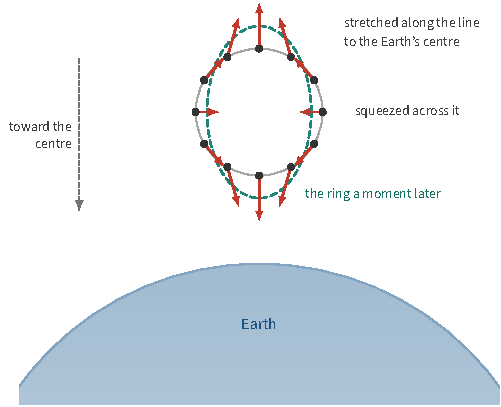
\includegraphics{ch02-tides}
\caption{Tides. A ring of freely falling particles above the Earth is
stretched along the direction to the Earth's centre and squeezed across it.
The arrows show the accelerations of the particles relative to the centre of
the ring.}
\label{fig:tides}
\end{figure}

In general relativity the relative acceleration of two nearby free-fall paths
separated by a small displacement $\xi^{\mu}$ is
\begin{equation}
  \frac{\dd^{2}\xi^{\mu}}{\dd\tau^{2}} = -R^{\mu}{}_{\alpha\nu\beta}\,u^{\alpha}\xi^{\nu}u^{\beta},
  \label{eq:geodesic-deviation}
\end{equation}
where $u^{\mu}$ is the four-velocity of the falling bodies and
$R^{\mu}{}_{\alpha\nu\beta}$ is the \emph{Riemann curvature tensor},
\begin{equation}
  \begin{split}
  R^{\mu}{}_{\alpha\nu\beta} = {}&\partial_{\nu}\Gamma^{\mu}{}_{\alpha\beta}
  - \partial_{\beta}\Gamma^{\mu}{}_{\alpha\nu}\\
  &+ \Gamma^{\mu}{}_{\nu\lambda}\Gamma^{\lambda}{}_{\alpha\beta}
  - \Gamma^{\mu}{}_{\beta\lambda}\Gamma^{\lambda}{}_{\alpha\nu}.
  \end{split}
  \label{eq:riemann}
\end{equation}
The Riemann tensor vanishes everywhere if and only if spacetime is flat. When
\cref{ex:flow} asked whether a metric describes flat spacetime, computing its
Riemann tensor would have answered directly, with no need to guess the right
change of coordinates.

In the weak-field limit, the tidal part of the Riemann tensor becomes the
familiar Newtonian tidal tensor, $R^{i}{}_{0j0} \approx \partial_{i}\partial_{j}\Phi$.
Near the Earth the stretching acceleration across a person \SI{2}{\metre} tall
is about $2GML/r^{3} \approx \SI{6e-6}{\metre\per\second\squared}$, far too
small to notice. Near a black hole of a few solar masses it would tear a person
apart. Tides are one of the first things a spacetime engineer checks on behalf
of a traveller.

\begin{checkpoint}[label=chk:tidal-volume]
A small ball of freely falling particles above the Earth is stretched along
the direction to the Earth's centre by a relative acceleration of $2GM/r^{3}$
per unit length, and squeezed along each of the two directions across it by
$GM/r^{3}$ per unit length. Does the volume of the ball begin to grow, to
shrink, or neither?
\end{checkpoint}

Two combinations of the Riemann tensor carry the information Einstein's
equation needs. The \emph{Ricci tensor} and the \emph{Ricci scalar} are
\begin{equation*}
  R_{\alpha\beta} = R^{\mu}{}_{\alpha\mu\beta}, \qquad R = g^{\alpha\beta}R_{\alpha\beta},
\end{equation*}
and the \emph{Einstein tensor} is
\begin{equation}
  G_{\alpha\beta} = R_{\alpha\beta} - \tfrac{1}{2}R\,g_{\alpha\beta}.
  \label{eq:einstein-tensor}
\end{equation}
The Einstein tensor is the \enquote{curvature of spacetime} on the left side of
Einstein's equation. \Cref{ch:matter-geometry} explains why this particular
combination appears, and uses it to compute what a geometry demands.

\begin{deeper}{tensors and coordinates}
The objects in this chapter are \emph{tensors}: quantities whose components
change in a definite way under a change of coordinates, so that an equation
between tensors holds in every coordinate system if it holds in one. The metric
is a symmetric tensor of type $(0,2)$ and the Riemann tensor has type $(1,3)$.
The Christoffel symbols are \emph{not} the components of a tensor, which is why
they can vanish at a point in one set of coordinates and not in another.
Spacetime is modelled as a four-dimensional Lorentzian manifold, and the sign
conventions here are those of Misner, Thorne and Wheeler; Wald develops the
same material in coordinate-free form.
\end{deeper}

\begin{revisited}{The windowless capsule}
Yes: they can look for tides. Near the Earth, two balls released a few metres
apart, one above the other, drift apart, with a relative acceleration of a few
millionths of a metre per second squared for every metre of separation. In a
minute, two balls released ten metres apart drift apart by a few
centimetres. In deep space the balls stay where they were
put. The relative acceleration is curvature, and no choice of frame removes
it. The equivalence principle holds only in a laboratory small enough, and an
experiment short enough, for tides to go unnoticed.
\end{revisited}

% ===========================================================================
\begin{chaptersummary}
\item With $c = 1$, time and distance share units and light moves at \ang{45}
  on a spacetime diagram.
\item The interval $\Delta s^{2} = -\Delta t^{2} + \Delta x^{2} + \Delta y^{2} + \Delta z^{2}$
  is the same for all inertial observers. It is timelike, null or spacelike,
  and light cones divide spacetime into what an event can and cannot
  influence.
\item A clock measures proper time $\tau = \int\sqrt{-\dd s^{2}}$ along its
  worldline. In flat spacetime the straight worldline between two events
  records the most proper time; in curved spacetime a free-fall worldline
  records more than every nearby worldline over any short enough stretch.
\item The metric $g_{\mu\nu}$ gives the interval between neighbouring events in
  any coordinates. Effects of the coordinates can be dramatic, as in flowing
  coordinates, where light's coordinate speed differs from 1.
\item In a weak field a clock runs at $\dd\tau/\dd t \approx 1 + \Phi - v^{2}/2$.
  Light climbing out of a potential arrives redshifted, because clocks at
  different heights tick at different rates. Near a black hole the rate of a
  clock held at rest falls to zero at the horizon.
\item The Schwarzschild geometry can be pictured as space flowing inward at the
  Newtonian escape speed; the horizon is where the flow reaches the speed of
  light. A clock held at rest is slowed by its motion upstream through the
  flow.
\item Free bodies follow geodesics, and the variation of clock rates from place
  to place acts as a gravitational field. The Riemann tensor measures tides,
  the true signature of curvature; the Ricci and Einstein tensors are built
  from it.
\end{chaptersummary}

\begin{checkanswers}
\item[\ref{chk:classify}] The probe covers 4 light-seconds in 5 seconds, at
  speed 0.8. Its clock records $\sqrt{5^{2} - 4^{2}} = 3$ seconds, since the
  interval $AC$ is timelike, $\Delta s^{2} = -25 + 16 = -9$. The interval $AB$
  is spacelike, $\Delta s^{2} = -9 + 16 = +7$, so no probe can be present at
  both. An observer who finds $A$ and $B$ simultaneous has $\Delta t' = 0$, and
  the invariance of the interval gives $\Delta x'^{2} = 7$: the events are
  $\sqrt{7} \approx 2.65$ light-seconds apart for that observer.
\item[\ref{chk:zigzag}] Zigzag back and forth at nearly the speed of light. On
  each leg $\dd\tau = \sqrt{1 - v^{2}}\,\dd t$, which approaches zero as $v \to 1$,
  so the total can be made as small as you like: at $v = 0.99$ the clock
  records 1.4 of the ten years. The limit, zero, belongs to light, which
  carries no clock. There is no worldline of least proper time, only one of
  greatest: the straight one, which records all ten years.
\item[\ref{chk:grid-clock}] With $\dd x = 0$,
  $\dd s^{2} = -(1 - v_{0}^{2})\,\dd t^{2} = -0.64\,\dd t^{2}$, so
  $\dd\tau = 0.8\,\dd t$: eight years. The grid point moves at speed 0.6 past
  the inertial observers whose clocks keep the time $t$, and
  $10\sqrt{1 - 0.6^{2}} = 8$ is exactly the time dilation of a clock moving at
  that speed. The metric has done the calculation of special relativity for
  us.
\item[\ref{chk:earth-centre}] Neither: the rate follows the potential $\Phi$,
  not the pull. Going down from the surface, the pull still points toward the
  centre, so $\Phi$ keeps falling all the way down. The centre is the bottom of
  the potential, and its clock is the slowest of the three. For an Earth of
  uniform density, $\Phi$ at the centre is 1.5 times its value at the surface,
  so the centre clock runs slow compared with a surface clock by
  $0.5\,GM/(c^{2}R) \approx 3.5\times10^{-10}$, about 11 milliseconds a year.
  The real Earth, denser toward its centre, gives somewhat more.
\item[\ref{chk:tidal-volume}] Neither. The volume's acceleration, as a
  fraction of the volume, is the sum of the relative accelerations per unit
  length along three perpendicular directions:
  $2GM/r^{3} - GM/r^{3} - GM/r^{3} = 0$. In empty space, tides change the shape
  of a ball of falling particles but, at first, not its volume. The sum is
  $-\nabla^{2}\Phi$, which vanishes wherever there is no matter;
  \cref{ch:matter-geometry} shows what matter does to it.
\end{checkanswers}

\begin{problems}
\item \diff{1} Two events are separated by $\Delta t = \SI{2}{\second}$ and
  $\Delta x = 1.5$~light-seconds. Find the interval and classify it. What proper
  time does a clock record if it travels between them at constant velocity?
\item \diff{2}\label{prob:simultaneity} \textbf{Whose now?} The crew of the ship
  in the Betelgeuse thought experiment flies past the Earth toward the star at
  speed 0.5. Using the Lorentz transformation $t' = \gamma(t - vx)$, show that
  for the crew the explosion happened about 318 years before they passed you.
  What would an observer flying away from Betelgeuse at the same speed say?
\item \diff{1} A clock travels at $v = 0.99$ for one year of Earth time. How much
  time does it record?
\item \diff{2} \textbf{Accelerating twin.} Repeat the twins' trip with a more
  realistic flight plan: the traveller accelerates uniformly from rest to $0.8$
  over the first year of Earth time, cruises, and decelerates symmetrically at
  the star and on the way home. Set up the proper-time integral and evaluate it
  numerically.
\item \diff{2}\label{prob:gps-curves} \textbf{The curves of \cref{fig:clock-offsets}.} For a
  clock on a circular orbit of radius $r$, show that its daily gain over a clock
  on the ground is proportional to $1/R - 3/(2r)$. At what orbital radius does it
  vanish? Plot the gain from height, the loss from speed and the net result.
\item \diff{2}\label{prob:neutron-star} \textbf{Neutron star.} Show that a clock
  on the surface of a neutron star of mass $1.4\,\Msun$ and radius
  \SI{12}{\kilo\metre} runs at 0.81 of the rate of a distant clock. Use
  $G\Msun/c^{2} = \SI{1.477}{\kilo\metre}$.
\item \diff{2} \textbf{Polar coordinates.} For the flat two-dimensional metric
  $\dd s^{2} = \dd r^{2} + r^{2}\dd\phi^{2}$, compute all the Christoffel symbols
  from \cref{eq:christoffel}. Show that the geodesic equation has straight lines
  as solutions.
\item \diff{2} \textbf{Flowing coordinates, again.} Compute the Christoffel
  symbols of \cref{eq:flow-metric} and show that the Riemann tensor vanishes.
  Then replace $v_{0}$ by a function $v(y)$ and show that the Riemann tensor no
  longer vanishes.
\item \diff{2}\label{prob:geodesic} \textbf{Deriving the geodesic equation.}
  Write the proper time along a worldline as
  $\tau = \int \sqrt{-g_{\mu\nu}\dot x^{\mu}\dot x^{\nu}}\,\dd\lambda$, where the dot
  is $\dd/\dd\lambda$. Apply the Euler--Lagrange equations and choose
  $\lambda = \tau$ to obtain \cref{eq:geodesic}.
\item \diff{2}\label{prob:thrown-ball} \textbf{The thrown ball.} A ball is thrown
  straight up at speed $v_{0}$ and caught at the same height. Using
  \cref{eq:clock-rate} with $\Phi = gh/c^{2}$, show that its clock gains
  $v_{0}^{3}/(3gc^{2})$ over a clock held at the height of the hand. Then show that
  any other path $h(t)$ with the same endpoints gains less.
\item \diff{3}\label{prob:orbit-paradox} \textbf{The orbit paradox.} An
  astronaut in a circular orbit of radius $r$ passes a colleague standing on
  top of a tower of the same height, and they meet again one orbit later.
  Using \cref{eq:clock-rate}, show that the colleague on the tower, who is not
  in free fall, records more time, by the fraction $GM/(2rc^{2})$, and find the
  difference over one orbit at the height of the space station,
  $r = \SI{6790}{\kilo\metre}$. Then resolve the paradox. (a)~Show that two
  circular orbits of the same radius, tilted slightly with respect to each
  other, cross again after half an orbit, so that a full orbit is longer than
  the \enquote{short enough stretch} of the key idea of
  \topicref{sec:geodesics}. (b)~Describe a third worldline, also in free fall,
  that joins the same two events and records more time than either.
\item \diff{2} \textbf{The river.} Show that \cref{eq:river} turns into
  \cref{eq:schwarzschild} under the change of time coordinate
  $\dd T = \dd t + \frac{\sqrt{r_{\mathrm{s}}/r}}{1 - r_{\mathrm{s}}/r}\,\dd r$.
\item \diff{3} \textbf{Tides near a black hole.} Estimate the stretching
  acceleration across a \SI{2}{\metre} tall person falling feet first into a black
  hole of $10\,\Msun$ at the moment they cross the horizon, and again for a black
  hole of $10^{9}\,\Msun$. Which one could a traveller cross unharmed, and why
  does the answer depend on the mass the way it does?
\end{problems}

\begin{furtherreading}
\item[\textcite{Hartle2003}] A physics-first introduction to general relativity
  that builds intuition for metrics, clocks and geodesics before the formalism.
\item[\textcite{Schutz2009}] A careful, gentle development of spacetime
  diagrams, tensors and curvature, well suited to self-study.
\item[\textcite{Carroll2004}] A graduate-level introduction that covers the
  geometry of this chapter with full mathematical care.
\item[\textcite{Misner1973}] The encyclopedic classic, with deep geometric
  intuition; its sign conventions are the ones used in this book.
\item[\textcite{Wald1984}] General relativity in coordinate-free form.
\item[\textcite{Ashby2003}] Relativity in satellite navigation, including the
  Earth's rotation and shape.
\item[\textcite{Pound1960}] The first laboratory measurement of the
  gravitational redshift, in a tower at Harvard.
\item[\textcite{Chou2010}] Clocks that detect a change of height of
  \SI{33}{\centi\metre}.
\item[\textcite{Hamilton2008}] The river model of black holes, developed in
  full.
\item[\textcite{Michell1784}] Michell's dark stars, the first discussion of
  objects from which light cannot escape.
\end{furtherreading}

% !TEX root = ../main.tex
\chapteropening{%
\Cref{ch:geometry} gave us the left side of Einstein's equation, the geometry.
This chapter supplies the right side, the description of matter, and then puts
the two together.

By the end of it you will be able to take any metric, compute the matter it
requires, and read the result the way a spacetime engineer does: as a list of
demands that some physical material would have to meet.}{%
\item describe the energy, momentum and stress of matter with the
  stress-energy tensor, and say what each component means;
\item compute the energy density that any observer measures;
\item write down the stress-energy of dust, fluids, radiation, tension and
  vacuum energy;
\item state Einstein's equation, convert between geometric and everyday units,
  and recover Newton's gravity from it;
\item carry out the spacetime engineer's central calculation, from a chosen
  metric to the matter it demands, and recognize the first signs of an exotic
  demand.}
\chapter{How Matter Shapes Spacetime}\label{ch:matter-geometry}

% ===========================================================================
\section{Energy depends on who measures it}\label{sec:energy-observers}

\begin{thought}{A brick in passing}
A brick sits on a table. You fly past it at 80 percent of the speed of light.
Because the brick moves relative to you, each of its atoms carries more energy
by the factor $\gamma = 1/\sqrt{1 - 0.8^{2}} = 5/3$. Is the energy per unit
volume that you measure larger by the same factor, or by a different one?
\end{thought}

In Newtonian physics, the mass of a brick is one fixed number. In relativity
the brick's \emph{energy} depends on the observer: someone moving past it sees
it carry kinetic energy as well as its rest energy. To describe matter in a
way every observer can use, we need to say how the measured energy changes
from one observer to another.

A particle of mass $m$ with four-velocity $u^{\mu}$ has \emph{four-momentum}
$p^{\mu} = m\,u^{\mu}$. An observer with four-velocity $w^{\mu}$ measures the
particle's energy to be
\begin{equation}
  E = -g_{\mu\nu}\,p^{\mu}w^{\nu} \equiv -p_{\mu}w^{\mu}.
  \label{eq:measured-energy}
\end{equation}
In the second form we have \emph{lowered an index}, $p_{\mu} = g_{\mu\nu}p^{\nu}$:
lowering indices with the metric is the bookkeeping that turns a pair of
vectors into a number every observer agrees on. For an observer at rest in flat
spacetime, $w^{\mu} = (1,0,0,0)$ and \cref{eq:measured-energy} gives
$E = p^{0}$. For a particle at rest relative to the observer, $E = m$, its rest
energy $mc^{2}$ in ordinary units.

A continuous material, such as a gas, a fluid or a stretched rope, needs more
than a four-momentum. At each event we want to know how much energy is present
per unit volume, how fast energy is flowing, how much momentum there is, and
what forces neighbouring parts of the material exert on each other. All of
this fits into one symmetric $4\times4$ array, the \emph{stress-energy tensor}
$T^{\mu\nu}$ (\cref{fig:stress-energy}). In the frame of a given observer,
$T^{tt}$ is the \textbf{energy density}; $T^{ti} = T^{it}$ is the
\textbf{energy flux} in direction $i$, which equals the density of momentum in
that direction; and $T^{ij}$ is the \textbf{stress}, the flux of $i$-momentum
across a surface facing the $j$ direction. The diagonal stresses are
\textbf{pressures} and the off-diagonal ones are \textbf{shear stresses}.

\begin{figure}[tb]
\centering
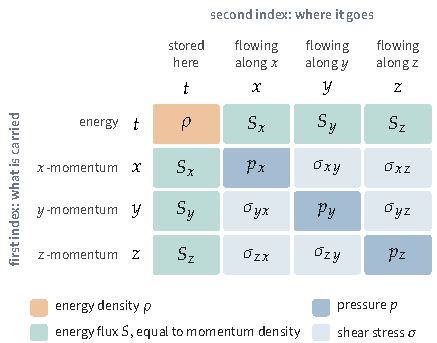
\includegraphics{ch03-stress-energy}
\caption{The components of the stress-energy tensor in one observer's frame.
The array is symmetric, so ten numbers describe the matter at each event.}
\label{fig:stress-energy}
\end{figure}

Observers in relative motion split the same tensor into energy, flux and
stress differently, just as they split an interval into time and distance
differently. The rule generalizes \cref{eq:measured-energy}: an observer with
four-velocity $w^{\mu}$ measures the energy density
\begin{equation}
  \rho_{w} = T_{\mu\nu}\,w^{\mu}w^{\nu},
  \label{eq:observed-density}
\end{equation}
where $T_{\mu\nu} = g_{\mu\alpha}g_{\nu\beta}T^{\alpha\beta}$ is the tensor
with both indices lowered. This formula is one of the most used in the book.
When a geometry demands matter, the first question is always what energy
density each observer would measure.

The simplest material is \textbf{dust}: particles at rest relative to one
another, with no pressure between them. In the dust's own rest frame the only
nonzero component is the energy density $\rho_{0}$, and the tensor that
reduces to that in the rest frame is
\begin{equation}
  T^{\mu\nu} = \rho_{0}\,u^{\mu}u^{\nu},
  \label{eq:dust}
\end{equation}
where $u^{\mu}$ is the dust's four-velocity.

\begin{example}[label=ex:tension-passing]{Tension seen in passing}
A long rod at rest has energy density $\rho_{0}$ and is stretched along its
length, the $x$ direction, by a tension $\tau$. In its rest frame
$T^{tt} = \rho_{0}$ and $T^{xx} = -\tau$ (a pull is a negative pressure), and
all other components vanish. What energy density does an observer moving
along the rod at speed $v$ measure?

\solution The observer's four-velocity is $w^{\mu} = \gamma\,(1, v, 0, 0)$. In
flat spacetime, lowering both indices leaves these two components unchanged:
$T_{tt} = \rho_{0}$ and $T_{xx} = -\tau$. \Cref{eq:observed-density} then gives
\begin{equation*}
  \rho_{w} = \gamma^{2}\bigl(T_{tt} + v^{2}\,T_{xx}\bigr)
  = \gamma^{2}\bigl(\rho_{0} - v^{2}\tau\bigr).
\end{equation*}

\discussion Tension lowers the energy density that a passing observer
measures. For ordinary materials the effect is tiny: the energy density
includes the rest energy, and for steel near its breaking point $\tau/\rho_{0}$
is about $10^{-12}$. But a material whose tension \emph{exceeded} its energy
density would look negative to observers moving fast enough along it, since
$\rho_{w} < 0$ whenever $v^{2} > \rho_{0}/\tau$. That is exactly the kind of
material Morris and Thorne found a wormhole throat needs.
\end{example}

\begin{checkpoint}[label=chk:laser]
A laser beam travelling along $+x$ has $T^{tt} = T^{tx} = T^{xt} = T^{xx} = u$,
with all other components zero. What energy density does an observer moving
along $x$ at speed $v$ measure? What does one moving at $0.8$ with the beam
measure, and one moving at $0.8$ against it?
\end{checkpoint}

\begin{revisited}{A brick in passing}
By more: the factor is $\gamma^{2}$. Each atom's energy is larger by $\gamma$,
and the brick is contracted along the direction of motion, which packs the
atoms more densely by another factor of $\gamma$. The formulas say the same
thing: with $T^{\mu\nu} = \rho_{0}u^{\mu}u^{\nu}$, \cref{eq:observed-density}
gives $\rho_{w} = \rho_{0}(u_{\mu}w^{\mu})^{2} = \gamma^{2}\rho_{0}$, because
$u_{\mu}w^{\mu} = -\gamma$ for two four-velocities in relative motion at speed
$v$. At 80 percent of the speed of light, $\gamma^{2} = 25/9 \approx 2.8$.
Energy density is not a quantity all observers share; it is one component of a
tensor, and each observer sees a different mix of components.
\end{revisited}

% ===========================================================================
\section{Pressure, tension and the vacuum}\label{sec:catalogue}

\begin{thought}{Flying through empty space}
Cosmologists have found that empty space seems to carry a small energy density
of its own, the \enquote{dark energy} that makes the expansion of the universe
speed up. When you flew past the brick, you measured more energy density than
someone at rest beside it. If you fly through empty space at 80 percent of the
speed of light, do you measure more of the vacuum's energy density too?
\end{thought}

The stress-energy tensors of a few kinds of matter recur throughout this book.
Each is simplest in its own rest frame.

\paragraph{Perfect fluid.} A fluid with energy density $\rho$ and the same
pressure $p$ in every direction has
\begin{equation}
  T^{\mu\nu} = (\rho + p)\,u^{\mu}u^{\nu} + p\,g^{\mu\nu},
  \label{eq:perfect-fluid}
\end{equation}
which in the rest frame is $\mathrm{diag}(\rho, p, p, p)$. Dust is a perfect fluid
with $p = 0$. Gases, liquids and the interiors of stars are perfect fluids to
a good approximation.

\paragraph{Radiation.} A gas of light moving in all directions is a perfect
fluid with $p = \rho/3$.

\paragraph{Tension.} Stretch a rope and each part pulls on its neighbours along
the rope. A pull is a negative pressure, so tension appears in $T^{\mu\nu}$ as a
\emph{negative} diagonal stress: a material under tension $\tau$ along $z$ has
$T^{zz} = -\tau$. Tension is one of the spacetime engineer's most important
ingredients, and you will meet it again and again in the demands of engineered
geometries.

\paragraph{Vacuum energy.} Empty space can carry an energy density
$\rho_{\text{vac}}$ of its own, with stress-energy
\begin{equation}
  T_{\mu\nu} = -\rho_{\text{vac}}\,g_{\mu\nu}.
  \label{eq:vacuum-energy}
\end{equation}
In its rest frame, if it can be said to have one, this is an energy density
$\rho_{\text{vac}}$ with pressure $p = -\rho_{\text{vac}}$ in every direction: a
tension equal to the energy density.

\begin{deeper}{the electromagnetic field}
In Heaviside--Lorentz units with $c = 1$, a magnetic field of strength $B$
along $z$ has energy density $B^{2}/2$, a pressure $+B^{2}/2$ across the field
lines ($T^{xx} = T^{yy}$), and a tension $B^{2}/2$ along them
($T^{zz} = -B^{2}/2$). Field lines behave like stretched elastic bands that
push sideways on one another. The tension along the field equals the energy
density: this is the largest tension the dominant energy condition of
Chapter~5 allows, and magnetic fields reach it exactly.
\end{deeper}

\begin{checkpoint}[label=chk:rho-p]
For dust, radiation, a perfect fluid with $p > 0$, and vacuum energy, compute
$\rho + p$. Which of them has $\rho + p = 0$? (In Chapter~5 you will see that
the sign of $\rho + p$ decides whether matter focuses light.)
\end{checkpoint}

\begin{revisited}{Flying through empty space}
No: every observer measures the same vacuum energy density. For any
four-velocity, \cref{eq:vacuum-energy} and \cref{eq:four-velocity} give
$\rho_{w} = -\rho_{\text{vac}}\,g_{\mu\nu}w^{\mu}w^{\nu} = \rho_{\text{vac}}$.
In the language of \cref{ex:tension-passing}, the vacuum's tension equals its
energy density, so the factor $\gamma^{2}(\rho - v^{2}\tau)$ becomes
$\gamma^{2}\rho_{\text{vac}}(1 - v^{2}) = \rho_{\text{vac}}$: the tension exactly
cancels the boost that made the brick look denser. That is why a vacuum energy
defines no preferred state of rest, as empty space should not.
\end{revisited}

% ===========================================================================
\section{Einstein's equation}\label{sec:einstein}

\begin{thought}{Between the Earth and the Moon}
Between the Earth and the Moon there is almost no matter at all, so the
stress-energy on the right side of Einstein's equation is zero there. Does the
equation then say that spacetime between them is flat? If it does, what steers
the Moon around its orbit, and what raises the tides in the Earth's oceans?
\end{thought}

Energy and momentum are conserved: whatever flows out of a small box must be
accounted for by a loss inside it. In flat spacetime this is the statement
\begin{equation}
  \partial_{\mu}T^{\mu\nu} = 0 .
  \label{eq:conservation-flat}
\end{equation}
Its $\nu = t$ component is the continuity equation for energy,
$\partial_{t}T^{tt} + \partial_{i}T^{it} = 0$; its three spatial components say
that momentum changes only through the stresses acting on a region. In curved
spacetime the partial derivative becomes the \emph{covariant} derivative
$\nabla_{\mu}$, which adds Christoffel-symbol terms: $\nabla_{\mu}T^{\mu\nu} = 0$.
Physically, matter then exchanges energy and momentum with the gravitational
field in a definite way, and the extra terms describe the exchange.

Einstein's equation is
\begin{equation}
  G_{\mu\nu} = \frac{8\pi G}{c^{4}}\,T_{\mu\nu},
  \label{eq:einstein-si}
\end{equation}
with $G_{\mu\nu}$ the Einstein tensor of \cref{eq:einstein-tensor}. There are ten
equations here, one for each independent component of the two symmetric
tensors.

\begin{deeper}{why the Einstein tensor?}
Whatever sits on the left side must be consistent with conservation of energy
and momentum on the right. The Einstein tensor has exactly this property: its
covariant divergence vanishes identically, $\nabla^{\mu}G_{\mu\nu} = 0$ for
\emph{every} metric, a result called the contracted Bianchi identity.
Einstein's equation therefore implies $\nabla^{\mu}T_{\mu\nu} = 0$
automatically. Apart from a term proportional to the metric itself, which acts
as vacuum energy, the Einstein tensor is essentially the only combination of
the metric and its first two derivatives with this property.
\end{deeper}

From now on we set $G = 1$ as well as $c = 1$, and Einstein's equation reads
\begin{equation}
  G_{\mu\nu} = 8\pi\,T_{\mu\nu}.
  \label{eq:einstein}
\end{equation}
In these \emph{geometric units} everything is measured in powers of length. A
mass $M$ becomes the length $GM/c^{2}$: the Sun is \SI{1.48}{\kilo\metre} and
the Earth \SI{4.4}{\milli\metre}. Curvature has units of one over length
squared, and so, by \cref{eq:einstein}, do energy density and stress. To
convert back, multiply a geometric energy density or stress, with lengths in
metres, by
\begin{equation}
  \frac{c^{4}}{G} = \SI{1.21e44}{\newton}
  \label{eq:conversion}
\end{equation}
to get joules per cubic metre, which are the same as pascals, and divide by
$c^{2}$ to express an energy density as a mass density. This one conversion
factor is the stiffness of spacetime from \cref{eq:stiffness}.

Einstein's equation also has a statement in plain words, due to John Baez and
Emory Bunn. Release a small ball of test particles, all at rest relative to
one another, and let them fall freely. Tides may at once begin to change the
ball's shape, and its volume $V$ begins to change at the rate
\begin{equation}
  \frac{\ddot V}{V} = -4\pi\,\bigl(\rho + p_{x} + p_{y} + p_{z}\bigr),
  \label{eq:ball}
\end{equation}
where the dots are derivatives with respect to the particles' proper time, and
the energy density and the three pressures are those at the centre of the
ball, measured by an observer at rest relative to it. Energy density makes the
ball shrink, and so does pressure. Required of every small ball, in every
state of motion, \cref{eq:ball} is equivalent to the whole of Einstein's
equation.

\begin{example}[label=ex:newtonian, unbreakable]{The Newtonian limit}
Show that for the weak-field metric \cref{eq:weak-field} with a static
potential $\Phi$, the $tt$ component of Einstein's equation reduces to Poisson's
equation of Newtonian gravity, $\nabla^{2}\Phi = 4\pi\rho$.

\solution Compute the Einstein tensor of \cref{eq:weak-field} to first order in
$\Phi$. The Christoffel symbols are first order, so their products in
\cref{eq:riemann} are second order and can be dropped. The calculation
(\cref{prob:weak-field}) gives $G_{tt} \approx 2\,\nabla^{2}\Phi$. For slowly
moving matter the dominant component of the stress-energy is the energy
density, $T_{tt} \approx \rho$, so $G_{tt} = 8\pi T_{tt}$ becomes
$\nabla^{2}\Phi = 4\pi\rho$: Poisson's equation, in units with $G = 1$.

\discussion Newtonian gravity is the weak-field, slow-motion limit of
Einstein's equation, and the factor $8\pi$ is what makes the limit come out
right. Einstein fixed the constant in just this way, by requiring his equation
to reproduce Newton's gravity wherever Newton's gravity works. Every
prediction beyond Newton, from the bending of starlight to the clock rates of
\cref{ch:geometry}, then came with no adjustable number left.
\end{example}

In empty space the right side of \cref{eq:ball} vanishes. A ball of falling
particles is still stretched and squeezed by tides, but its volume does not
begin to change: the stretching along one direction is balanced by squeezing
along the others, as you found for the Earth in \cref{chk:tidal-volume}. In
Newtonian terms, Poisson's equation in empty space says $\nabla^{2}\Phi = 0$,
not $\Phi = 0$. In the full theory, the trace of Einstein's equation gives
$R = -8\pi T$, with $T = g^{\mu\nu}T_{\mu\nu}$, so in empty space $R = 0$ and
then $G_{\mu\nu} = 0$ says $R_{\mu\nu} = 0$. The Ricci tensor, which governs
changes of volume, vanishes. The Riemann tensor, with twenty independent
components to the Ricci tensor's ten, need not; the rest of the curvature is
set by matter elsewhere and by what arrives from far away.

\begin{checkpoint}[label=chk:water]
Water has a density of \SI{1000}{\kilogram\per\cubic\metre}. What is its
energy density in geometric units? Einstein's equation then sets a curvature
of order $8\pi\rho$; over what distance does spacetime filled with water curve
appreciably?
\end{checkpoint}

\begin{revisited}{Between the Earth and the Moon}
No. Einstein's equation fixes only part of the curvature. Where there is no
matter it sets the Ricci tensor to zero, so a ball of falling particles keeps
its volume at first, but the rest of the Riemann tensor survives. In Newtonian
terms, the potential between the Earth and the Moon obeys $\nabla^{2}\Phi = 0$
without being zero: its slope steers the Moon around its orbit, and its second
derivatives, which add up to zero, stretch the oceans along the line to the
Moon and squeeze them across it. Empty space can be curved. Matter is what
makes a falling ball begin to shrink.
\end{revisited}

% ===========================================================================
\section{Pressure gravitates}\label{sec:pressure}

\begin{thought}{A box of hot gas}
Inside a star, pressure adds to the source of gravity. Take a sealed steel box
of gas and heat it until the pressure inside is enormous, while the box keeps
its shape. Does the box now pull on a distant planet harder than its energy
alone would suggest, because of all that pressure?
\end{thought}

Einstein's equation says more than Newton's. In a perfect fluid at rest the
three pressures are equal, so by \cref{eq:ball} a small ball of test particles
begins to shrink at a rate set by
\begin{equation}
  \rho + 3p ,
  \label{eq:active-mass}
\end{equation}
and this is the quantity that plays the role of $\rho$ in Poisson's equation
(\cref{prob:rho-3p}).
Pressure is a source of gravity alongside energy. For ordinary matter the
pressure is tiny compared with the energy density, which includes the rest
energy $mc^{2}$, so Newton never noticed. Tension, however, \emph{weakens}
gravity, and enough of it reverses its sign. Vacuum energy has
$\rho + 3p = -2\rho_{\text{vac}}$: it repels. This is why a positive vacuum
energy makes the expansion of the universe accelerate, and it is a first hint
of what engineered spacetimes can do with tension.

\begin{keyidea}
In general relativity every component of the stress-energy tensor bends
spacetime: energy, momentum and stress alike. Pressure attracts, tension
repels, and a spacetime engineer designs with all of them.
\end{keyidea}

\begin{checkpoint}[label=chk:stop-tension]
A material has energy density $\rho$ and the same stress $p$ in every
direction. What value of $p$ would keep a small ball of test particles inside
it from beginning to shrink? Is that a pressure or a tension?
\end{checkpoint}

\begin{figure}[tb]
\centering
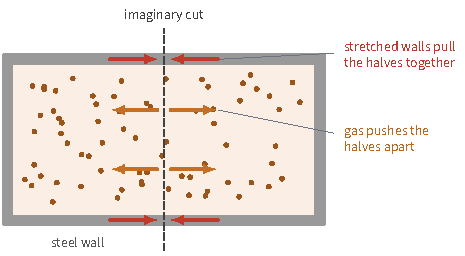
\includegraphics{ch03-gas-box}
\caption{A sealed box of hot gas, cut by an imaginary plane. Across the cut,
the gas pushes the two halves apart and the stretched walls pull them
together. In equilibrium the forces balance, for every cut.}
\label{fig:gas-box}
\end{figure}

\begin{revisited}{A box of hot gas}
No. The gas pressure does add $3p$ to the source of gravity inside the box,
but the steel walls that hold the gas in are under tension, and tension
subtracts. For any object that holds itself together in equilibrium, the two
cancel exactly. Cut the box in two with an imaginary plane
(\cref{fig:gas-box}). The gas pushes the halves apart with a force equal to its
pressure times the area of gas in the cut, and the walls pull them together
with their tension times the area of steel in the cut. Equilibrium means these
balance, for every cut in every direction, so the total of all the stresses
over the box, $\int (T^{xx} + T^{yy} + T^{zz})\,\dd V$, is zero
(\cref{prob:von-laue}). A distant planet feels only the box's total energy,
which heating has raised by the thermal energy added, $\Delta E$, making the
box heavier by $\Delta E/c^{2}$.
\end{revisited}

% ===========================================================================
\section{Reading the equation backwards}\label{sec:backwards}

\begin{thought}{A room where time runs fast}
In a rocket accelerating through empty space, clocks at the nose tick faster
than clocks at the tail, and nothing but the rocket's acceleration is needed to
make it so. Could you instead arrange for clocks to tick fastest in the middle
of a room and slower toward both walls, keeping the room's space perfectly
flat? What would have to fill the room?
\end{thought}

Here is the spacetime engineer's central calculation. It has five steps.
\begin{enumerate}
\item Write down the metric $g_{\mu\nu}$ of the geometry you want.
\item Compute the Christoffel symbols, \cref{eq:christoffel}.
\item Compute the Riemann tensor \cref{eq:riemann}, then the Ricci tensor, the
  Ricci scalar and the Einstein tensor \cref{eq:einstein-tensor}.
\item Read off the demanded stress-energy, $T_{\mu\nu} = G_{\mu\nu}/8\pi$.
\item Interpret it: compute the energy density and stresses measured by the
  observers you care about, using \cref{eq:observed-density}.
\end{enumerate}
For all but the simplest metrics, steps 2 and 3 are best done with computer
algebra. The examples in this chapter are simple enough to follow by hand, and
each teaches something the rest of the book builds on.

\begin{example}[label=ex:lapse, unbreakable]{Clocks that run at different rates}
Suppose we want clocks to run at different rates at different places along
$x$, while space itself stays exactly flat. The metric is
\begin{equation}
  \dd s^{2} = -\alpha(x)^{2}\,\dd t^{2} + \dd x^{2} + \dd y^{2} + \dd z^{2},
  \label{eq:lapse-metric}
\end{equation}
where $\alpha(x) > 0$ is the rate of a clock at rest at $x$, relative to
coordinate time. Find the matter this geometry demands.

\solution \emph{Christoffel symbols.} Only $g_{tt} = -\alpha^{2}$ varies, and
only with $x$. Writing $\alpha' = \dd\alpha/\dd x$, \cref{eq:christoffel} gives
two independent nonzero symbols:
\begin{equation*}
  \Gamma^{t}{}_{tx} = \Gamma^{t}{}_{xt} = \frac{\alpha'}{\alpha},
  \qquad
  \Gamma^{x}{}_{tt} = \alpha\,\alpha' .
\end{equation*}
\emph{Curvature.} From \cref{eq:riemann}, the nonzero components of the Ricci
tensor are
\begin{equation*}
  R_{tt} = \alpha\,\alpha'', \qquad R_{xx} = -\frac{\alpha''}{\alpha},
\end{equation*}
and the Ricci scalar is $R = g^{tt}R_{tt} + g^{xx}R_{xx} = -2\alpha''/\alpha$.
\emph{Einstein tensor.} From \cref{eq:einstein-tensor}, $G_{tt} = 0$ and
$G_{xx} = 0$, while
\begin{equation*}
  G_{yy} = G_{zz} = -\tfrac{1}{2}R = \frac{\alpha''}{\alpha}.
\end{equation*}
\emph{Interpretation.} A clock at rest at $x$ has four-velocity
$w^{\mu} = (1/\alpha, 0, 0, 0)$, and by \cref{eq:observed-density} it measures
energy density $\rho = G_{tt}/(8\pi\alpha^{2}) = 0$. The demand is
\begin{equation}
  \rho = 0, \quad p_{x} = 0, \quad p_{y} = p_{z} = \frac{\alpha''}{8\pi\,\alpha}.
  \label{eq:lapse-demand}
\end{equation}

\discussion Changing the rate of clocks from place to place, with space kept
flat, demands \emph{no energy at all}: only stress, and only in the directions
perpendicular to the change. If $\alpha$ is a straight line, $\alpha = 1 + gx$,
the demand vanishes entirely: that geometry is flat spacetime seen by an
observer with constant acceleration $g$ (\cref{prob:rindler}), the rocket of
the thought experiment.
\end{example}

The Earth also makes clocks run at different rates at different heights, yet
the empty space around it holds no stress. The difference is that the Earth's
geometry curves space as well: the factor $(1 - 2\Phi)$ in front of the
spatial part of \cref{eq:weak-field}. In empty space the curvature of space and
the variation of clock rates cancel exactly in Einstein's equation
(\cref{prob:weak-field}). In \cref{ex:lapse} we insisted on keeping space flat,
and the stress is the price of that choice. Designs make choices like this all
the time, and Einstein's equation prices each one.

The price is steep. Take a clock rate that changes by one part in a billion
across one metre, so that $\alpha'' \sim \SI{e-9}{\per\metre\squared}$. By
\cref{eq:lapse-demand,eq:conversion}, the stress is about
$10^{-9}/(8\pi) \times \SI{1.2e44}{\pascal} \approx \SI{5e33}{\pascal}$, the
pressure deep inside a neutron star, demanded to make two clocks a metre apart
differ by one part in a billion.

\begin{figure}[tb]
\centering
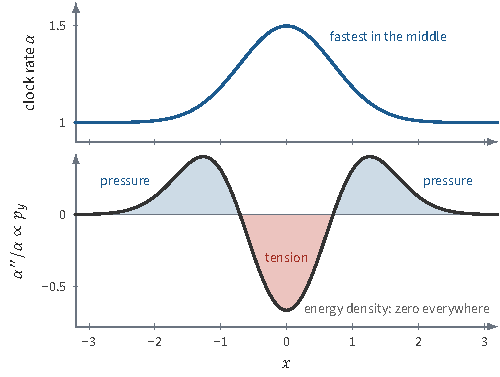
\includegraphics{ch03-lapse-bump}
\caption{Clocks that run fastest in the middle, $\alpha = 1 + \tfrac12
e^{-x^{2}}$ (top), and the stress this demands across the direction of the
change, \cref{eq:lapse-demand} (bottom). Around the peak the demand is a
tension; on the flanks it is a pressure. The energy density is zero
everywhere.}
\label{fig:lapse-bump}
\end{figure}

\begin{checkpoint}[label=chk:lapse-dip]
Suppose instead that clocks run \emph{slowest} in the middle, with
$\alpha = 1 - \tfrac12 e^{-x^{2}}$. Where is the demand a tension, and where a
pressure?
\end{checkpoint}

\begin{revisited}{A room where time runs fast}
The room must hold a strange material: one with no energy density at all, but
with stress along the two directions parallel to the walls
(\cref{fig:lapse-bump}). Where the clock rate peaks, $\alpha'' < 0$ and the
stress is a tension; nearer the walls, where $\alpha$ curves back up, it is a
pressure. The rocket needed nothing because its $\alpha$ is a straight line;
the room pays for the curvature of $\alpha$. And the tension at the peak is
worse than it looks. For light travelling parallel to the walls,
$\rho + p_{y} = \alpha''/(8\pi\alpha) < 0$, and in Chapter~5 you will learn that
ordinary matter always has $\rho + p \ge 0$ along every direction light can
travel. A simple bump in the rate of clocks already demands matter that no
ordinary material can provide.
\end{revisited}

% ===========================================================================
\section{When space flows unevenly}\label{sec:shear}

\begin{thought}{A river with a fast lane}
In \cref{ch:geometry}, space flowing at one uniform speed turned out to be flat
spacetime in disguise, and it cost nothing. Now let the flow run faster down
the middle of a channel than near its banks, the way a river does. Does that
cost anything? If it does, will the observers carried along by the flow
measure a positive or a negative energy density? Make a guess before reading
on.
\end{thought}

\begin{example}[label=ex:shear]{A flow of space that shears}
Let the speed of the flow of \cref{ex:flow} vary across space:
\begin{equation}
  \dd s^{2} = -\dd t^{2} + \bigl(\dd x + \beta(y)\,\dd t\bigr)^{2} + \dd y^{2} + \dd z^{2},
  \label{eq:shear-metric}
\end{equation}
a flow of space along $x$ whose speed depends on $y$. Find the energy density
measured by observers carried along by the flow.

\solution Observers carried by the flow move with $\dd x/\dd t = -\beta$ and
feel no force. Their four-velocity is $w^{\mu} = (1, -\beta, 0, 0)$, which
satisfies $g_{\mu\nu}w^{\mu}w^{\nu} = -1$ (\cref{prob:shear-check}). Carrying
out the recipe for \cref{eq:shear-metric} is longer than for \cref{ex:lapse},
and a good exercise for computer algebra (\cref{prob:shear-check}). The energy
density these observers measure is
\begin{equation}
  \rho = T_{\mu\nu}w^{\mu}w^{\nu} = -\frac{1}{32\pi}\left(\frac{\dd\beta}{\dd y}\right)^{2}.
  \label{eq:shear-density}
\end{equation}

\discussion Where the flow is uniform, $\dd\beta/\dd y = 0$ and nothing is
demanded, just as in \cref{ex:flow}. Wherever the flow shears, the observers
riding it measure a \emph{negative} energy density, whichever way the shear
goes, since the derivative is squared.
\end{example}

The numbers are once again enormous. A flow that changes from zero to the speed
of light across one metre has $\dd\beta/\dd y \approx \SI{1}{\per\metre}$, and
\cref{eq:shear-density,eq:conversion} give an energy density of about
\SI{-1.2e42}{\joule\per\cubic\metre}, equivalent to a mass density of about
\SI{-1e25}{\kilogram\per\cubic\metre}. Nuclear matter, the densest material in
nature, has about \SI{+2e17}{\kilogram\per\cubic\metre}.

\begin{checkpoint}[label=chk:shear-width]
Suppose the flow speed in \cref{ex:shear} rises steadily from $0$ to
$\beta_{0}$ across a layer of width $w$. What energy density do the riding
observers measure in the layer? If you make the layer twice as wide, what
happens to the energy density, and to the total negative energy in the layer
per unit area of its face?
\end{checkpoint}

\begin{revisited}{A river with a fast lane}
It costs a great deal, and the cost is negative energy. By
\cref{eq:shear-density}, observers riding a shearing flow of space measure
$\rho = -(\dd\beta/\dd y)^{2}/32\pi$, negative whichever way the shear runs.
This is the warp drive's problem in miniature. At the wall of a warp bubble the
flow of space changes from the bubble's speed to zero, so the wall is a region
of shear, and \cref{eq:shear-density} is why Alcubierre's bubble demands
negative energy there (\cref{fig:warp}b).
\end{revisited}

% ===========================================================================
\section{Every geometry has a price}\label{sec:price}

The recipe of \topicref{sec:backwards} never fails. Every metric you can write
down has an Einstein tensor, so every geometry has a demanded stress-energy.
Read backwards, Einstein's equation is a price list: it tells you exactly what
matter any geometry would require.

Whether anything in nature can pay the price is a separate question, and it is
the question the rest of this book is organized around. The examples of this
chapter already show its shape. Shaping the rate of clocks demands stress
without energy, and can demand matter that violates $\rho + p \ge 0$. Shearing
the flow of space demands negative energy density. Chapter~4 splits spacetime
into space and time the way these examples suggest, with a \emph{lapse} that
sets the rate of clocks and a \emph{shift} that describes the flow of space, and
shows how to compute demands like these efficiently. Chapter~5 states precisely
which demands ordinary matter can meet, and Chapter~6 asks how far quantum
physics can go beyond them.

% ===========================================================================
\begin{chaptersummary}
\item Energy depends on the observer. An observer with four-velocity $w^{\mu}$
  measures the energy density $\rho_{w} = T_{\mu\nu}w^{\mu}w^{\nu}$; a passing
  observer sees a brick's energy density raised by $\gamma^{2}$.
\item The stress-energy tensor $T^{\mu\nu}$ collects energy density, energy
  flux, momentum density and stress into one symmetric array.
\item Dust, perfect fluids, radiation, tension and vacuum energy each have a
  characteristic stress-energy. Tension is negative pressure, and it lowers the
  energy density that passing observers measure.
\item Einstein's equation $G_{\mu\nu} = 8\pi T_{\mu\nu}$ (with $G = c = 1$) links
  curvature to matter. Multiply geometric stresses by
  $c^{4}/G = \SI{1.21e44}{\newton}$ to get pascals.
\item In plain words, Einstein's equation says that a small ball of test
  particles, initially at rest relative to one another, begins to change
  volume at the rate $\ddot V/V = -4\pi(\rho + p_{x} + p_{y} + p_{z})$. In empty
  space $R_{\mu\nu} = 0$: tides remain, but they change only the ball's shape.
\item Newton's gravity is the weak-field limit. Beyond it, pressure gravitates
  through $\rho + 3p$ and tension can make gravity repel; in a body that holds
  itself together, the pressures and tensions cancel in total.
\item Reading the equation backwards gives the matter any geometry demands.
  Varying clock rates across flat space demands stress without energy; a
  shearing flow of space demands negative energy density.
\end{chaptersummary}

\begin{checkanswers}
\item[\ref{chk:laser}] Lowering the indices flips the sign of each component
  with a single $t$: $T_{tt} = T_{xx} = u$ and $T_{tx} = T_{xt} = -u$. With
  $w^{\mu} = \gamma\,(1, v, 0, 0)$,
  $\rho_{w} = \gamma^{2}u\,(1 - 2v + v^{2}) = u\,(1 - v)/(1 + v)$. Chasing the
  beam at $0.8$ gives $u/9$; running into it ($v = -0.8$) gives $9u$. Each
  photon is Doppler shifted by the factor $\sqrt{(1 - v)/(1 + v)}$, and the
  photons' number density changes by the same factor.
\item[\ref{chk:rho-p}] Dust: $\rho + p = \rho$. Radiation: $\rho + p = \tfrac43\rho$.
  Fluid with $p > 0$: $\rho + p > \rho$. Vacuum energy: $\rho + p = 0$. Only
  vacuum energy sits exactly on the boundary.
\item[\ref{chk:water}] $\rho = G\rho_{\mathrm{mass}}/c^{2} = 6.67\times10^{-11}
  \times 1000/(9.0\times10^{16}) \approx \SI{7.4e-25}{\per\square\metre}$. A
  curvature of $8\pi\rho$ corresponds to a length
  $1/\sqrt{8\pi\rho} \approx \SI{2e11}{\metre}$, more than the distance from
  the Earth to the Sun. Spacetime is stiff.
\item[\ref{chk:stop-tension}] By \cref{eq:ball} the ball keeps its volume when
  $\rho + 3p = 0$, that is, $p = -\rho/3$: a tension of one third of the
  energy density in every direction. Vacuum energy, with $p = -\rho$, goes
  beyond this, and a ball of test particles in it begins to grow.
\item[\ref{chk:lapse-dip}] Now $\alpha'' > 0$ near $x = 0$, so the demand there
  is a pressure; on the flanks, where $\alpha$ curves back toward 1 from
  below, it is a tension. Wherever the demand is a tension, $\rho + p_{y} < 0$.
\item[\ref{chk:shear-width}] In the layer $\dd\beta/\dd y = \beta_{0}/w$, so
  $\rho = -\beta_{0}^{2}/(32\pi w^{2})$. Doubling $w$ divides the energy
  density by four. The layer then holds twice the volume, so the total per
  unit area, $-\beta_{0}^{2}/(32\pi w)$, is halved. Thin layers of shear are
  expensive on both counts.
\end{checkanswers}

\begin{problems}
\item \diff{1} A cloud of dust with rest-frame density $\rho_{0}$ moves at speed
  $v$ along $y$. Write down all components of $T^{\mu\nu}$ in the observer's
  frame.
\item \diff{1} \textbf{Geometric units.} Express the mass of the Earth, the Sun
  and a $10^{9}\,\Msun$ black hole in metres. What energy density, in joules per
  cubic metre, corresponds to a geometric energy density of
  \SI{1}{\per\square\kilo\metre}?
\item \diff{2} \textbf{Magnetic tension.} Using the stress-energy of a magnetic
  field in the \emph{Going deeper} box on the electromagnetic field, verify
  that $\rho + p \ge 0$ for every direction of the pressure, and that the tension
  along the field lines equals the energy density.
\item \diff{2} \textbf{Vacuum energy.} Show from \cref{eq:vacuum-energy} that
  every observer measures the same energy density $\rho_{\text{vac}}$, and that
  the pressure is $-\rho_{\text{vac}}$ in every direction.
\item \diff{2}\label{prob:rho-3p} \textbf{Pressure gravitates.} Einstein's
  equation can be rewritten as
  $R_{\mu\nu} = 8\pi\bigl(T_{\mu\nu} - \tfrac12 T g_{\mu\nu}\bigr)$, with
  $T = g^{\mu\nu}T_{\mu\nu}$. For a perfect fluid at rest, show that
  $R_{tt} = 4\pi(\rho + 3p)$. Given that $R_{tt} \approx \nabla^{2}\Phi$ in a weak,
  static field, explain why $\rho + 3p$ plays the role of $\rho$ in Poisson's
  equation.
\item \diff{3}\label{prob:von-laue} \textbf{Stresses in a body at rest.} For a
  static body of finite size in flat spacetime, conservation gives
  $\partial_{j}T^{ij} = 0$. Show that $\int T^{xx}\,\dd V = 0$ by integrating
  $\partial_{j}(x\,T^{xj}) = T^{xx}$ over a region enclosing the body, and deduce
  that the pressures and tensions in the box of hot gas cancel in total.
\item \diff{2}\label{prob:weak-field} \textbf{Weak fields.} Compute the Einstein
  tensor of \cref{eq:weak-field} to first order in $\Phi$. Show that
  $G_{tt} \approx 2\nabla^{2}\Phi$, and that all components vanish where
  $\nabla^{2}\Phi = 0$. Explain why the result differs from \cref{ex:lapse}.
\item \diff{2}\label{prob:rindler} \textbf{Uniform acceleration.} Show that the
  metric \cref{eq:lapse-metric} with $\alpha = 1 + gx$ has vanishing Riemann
  tensor. What does an observer at rest at fixed $x$ feel?
\item \diff{2} \textbf{A rippled clock rate.} Take $\alpha = 1 + \epsilon\sin kx$
  with $0 < \epsilon < 1$ in \cref{ex:lapse}. Where is the demand a tension? For
  light moving along $y$, where is $\rho + p_{y}$ negative?
\item \diff{3}\label{prob:shear-check} \textbf{The shearing flow.} Using a
  computer algebra system, compute the Einstein tensor of \cref{eq:shear-metric}
  and verify \cref{eq:shear-density}. Check that $w^{\mu} = (1,-\beta,0,0)$ is a
  unit timelike vector. Then compute the energy density measured by an observer
  at rest in the coordinates, $w^{\mu} = (1,0,0,0)/\sqrt{1-\beta^{2}}$, where
  $|\beta| < 1$, and compare.
\item \diff{3} \textbf{Designing a fast-clock region.} You want a region where
  clocks run twice as fast as clocks far away, with space kept flat and the
  transition taking place over \SI{10}{\metre}. Using \cref{ex:lapse}, sketch a
  suitable $\alpha(x)$, locate the tensions and pressures it demands, and
  estimate their size in pascals.
\end{problems}

\begin{furtherreading}
\item[\textcite{Schutz2009}] A careful introduction to the stress-energy tensor
  through dust and perfect fluids.
\item[\textcite{Baez2005}] Einstein's equation stated through a ball of
  falling particles, the form used in this chapter, with its consequences
  worked out at an introductory level.
\item[\textcite{Carroll2004}] Einstein's equation, its Newtonian limit and the
  Bianchi identity at graduate level.
\item[\textcite{Hartle2003}] A physical approach to Einstein's equation and to
  what curvature does.
\item[\textcite{Misner1973}] The stress-energy tensor, and why stresses must
  balance in a body at rest.
\item[\textcite{Morris1988a}] The engineer's calculation of this chapter,
  applied to traversable wormholes.
\item[\textcite{Alcubierre1994}] The original warp drive. After \cref{ex:shear}
  you can follow its energy density calculation.
\end{furtherreading}


\backmatter
\printbibliography[heading=bibintoc,title={References}]
\printindex

\end{document}
